\documentclass[11pt,a4paper]{article}

% =====================================================================
% SPINE POSITION --- P16 (NEW), THE COSMOGENESIS SYNTHESIS PAPER.
%   Follows the cosmology (renumbered P15) and the matter sector (P14);
%   pulls the corpus's deductively forced consequences onto one problem
%   --- the cosmogenesis of matter across the one branch-point crossing --- and
%   carries it to a quantitative, falsifiable edge: the primordial
%   light-element abundances. The geometric-core border paper wraps the
%   enlarged whole as p0/17.
%
% CANON NOTE --- LIVE OPERATING PHILOSOPHY
%
% [†ONT-COSMO] COSMOLOGICAL GROUNDING --- hold this whenever a derivation runs.
%   The forced model (NOT an FLRW default) is stated whole in
%   ONTOLOGY_FOUNDATION_INDEX.md §1b. In one breath: the OBSERVABLE rate is
%   radiation-free sinh^{2/3} (Nariai proper frame, fixed by Λ, read LEFTWARD --
%   radiation and matter are inherited content read off the clock, never terms
%   that source the rate; no radiation-dominated era in the observable rate);
%   the PROGENITOR/local dynamics is ordinary GR at the standard Friedmann rate
%   (where the thermodynamics and BBN run, below the T_onset≈1.6 eV onset); the
%   two regimes are DISTINCT. THE BEGINNING IS THE BRANCH POINT r=0 (r2123). Do not conflate
%   them (the "~300x slower BBN" veer). The branch point is finite curvature: the
%   throat IS alpha, the substrate's defining constant; the r-chart divergence is the areal
%   coordinate degenerating. The seams are the two unit-speed loci r=-2a/sqrt3 and
%   r=+a/sqrt3. WHERE THE L1/L2 BOUNDARY LIES IS OPEN (THE_CLOSURE_LEDGER r2118).
%
% [†ONT-BANG] HOME --- the Big Bang as a forced synthesis, and the light elements
%   produced (ONTOLOGY_FOUNDATION_INDEX.md §1s). Masthead: the Big Bang is the
%   CONJUNCTION of eight established corpus results (the synthesis spine), not a
%   posit -- recognition, not proposal. TWO RATES ARE DIFFERENT OBJECTS (window =
%   leaf-level, radiation-included; observable = foliation-level, radiation-free):
%   no seam decoupling mechanism is demanded, and carrying either law into the
%   other's domain is quantitatively fatal (the ~300x veer / the re-manufactured
%   Hubble tension). The peak clears the deuterium bottleneck for EVERY progenitor
%   by the M-independent infall energy -- rho_hor is a FLOOR, not a peak (the r876
%   mass-ceiling was the artefact of reading the horizon-crossing average as the
%   peak). The cooling leg IS a standard BBN: He-4 and D produced at observed, the
%   composition fixed by the inherited baryon-to-photon ratio eta -- a SECOND datum of
%   the same handover, distinct from the radiation amplitude rho_r/rho_m that sets the
%   acoustic SCALE (P15); eta fixes the abundances and the CMB peak HEIGHTS, rho_r/rho_m
%   the peak SPACING. Li-7 the SHARED standard problem (synthesis, not
%   inheritance -- the corrected reading). Coherence, not correspondence; the open
%   edge is the full multi-abundance likelihood.
%
% CR is ONTOLOGICAL, not merely representational. "Reassignment / seam /
% inherited / lap / conjugate branch" are statements about a real geometry
% and a real previous universe's collapse. "Manufactured/shadow/projection/
% perspectival" mean built-by-construction-and-REAL, never unreal.
%
% REGISTER: recognition, not proposal. The field equations are Einstein's,
% unchanged; the nuclear reactions are the ordinary ones; only the reading
% --- that the hot dense era is the re-expansion of the previous universe's
% collapsed matter --- is CR's. The thesis is NOT "CR modifies BBN" but
% "the Big Bang is the deductively forced synthesis of consequences the
% corpus already establishes, and on it the observed light-element pattern
% is PRODUCED by an ordinary standard-rate nucleosynthesis run on the
% collapse's heat-turnaround-cool history."
%
% STATUS (honest, carried in-prose, not as tags):
%   ESTABLISHED (grounded, receipts in the corpus): the synthesis spine
%     (each arrow a prior paper's result); the seam is finite-curvature
%     and the reassignment is the kappa=0 identity (P7, P8); the effective
%     nuclear-window rate is the standard Friedmann rate (Sec rate); BBN is
%     time-reversal violating, so a freeze-out lives only on the cooling
%     leg (Sec trev); the infalling matter compresses adiabatically
%     (photons trapped) and its peak is bounded below by the M-independent
%     infall scale ~1e2 MeV >> T_D, dissociation guaranteed for every
%     progenitor (Sec peak); the cooling leg is a
%     standard BBN, giving He-4 and D at observed with one inherited eta
%     (Sec network).
%   BUILT (r955-r957, updated r967): the synthesis reading over the inheritance
%     reading --- the concrete thermodynamics (Sec peak) forces synthesis,
%     which is what makes lithium a SHARED problem rather than dissolved;
%     the exact abundances ARE NOW computed through a full multi-nuclide network
%     with CR's rate per epoch (Sec network; D/He-4 within 1sigma, StarLib-precise,
%     receipts computations/p16_bbn/). Remaining open edge = last-percent rate
%     precision + the derivation (vs inheritance) of eta -- both above the title's bar.
%   OPEN, named: the derivation (as against inheritance) of eta and the
%     progenitor spectrum; the full multi-abundance likelihood; whether one
%     progenitor handover fits D, He-4 AND the metallicity floor together.
%
% CORRECTION THIS PAPER CARRIES: the cosmology paper (P15) is to be brought
%   into the SYNTHESIS reading. Its "no in-situ nucleosynthesis / composition
%   inherited / lithium problem dissolved" is the observable-onset reading;
%   the deep re-expansion from the peak down through the bottleneck DOES the
%   nucleosynthesis, so lithium-7 carries the standard threefold
%   over-prediction --- the SAME problem as flat LCDM, neither dissolved nor
%   worsened. Deuterium moves from "sharp open constraint" to "produced at
%   observed." He-4 unchanged.
% =====================================================================

\usepackage[margin=1in]{geometry}
\usepackage{amsmath, amssymb, amsthm}
\usepackage{mathtools}
\usepackage{mathrsfs}
\usepackage{graphicx}
\usepackage[dvipsnames]{xcolor}
\usepackage{hyperref}
\usepackage{caption}
\usepackage{receipts}
\captionsetup{font=small, labelfont=bf}

\theoremstyle{plain}
\newtheorem{theorem}{Theorem}
\newtheorem{proposition}{Proposition}
\newtheorem{lemma}{Lemma}
\theoremstyle{definition}
\newtheorem{definition}{Definition}
\theoremstyle{remark}
\newtheorem{remark}{Remark}

\newcommand{\so}{\mathfrak{so}}
\newcommand{\dS}{\mathrm{dS}}
\newcommand{\rs}{r_{\mathrm{s}}}
\newcommand{\Mpl}{M_{\mathrm{Pl}}}
\newcommand{\TD}{T_{\mathrm{D}}}
\newcommand{\Tpk}{T_{\mathrm{peak}}}

\title{Cosmogenesis:\\
\large the Big Bang as a synthesis of Cosmological Relativity's deductively forced\\
consequences, and the primordial light-element abundances it produces}
\author{Daryl Janzen\\
\small Department of Physics and Engineering Physics\\
\small University of Saskatchewan}
\date{}

\begin{document}
\maketitle

\begin{abstract}
In Cosmological Relativity (CR) the cosmic beginning is not a singular origin but a
\emph{cosmogenesis}: the collapse of matter in a previous universe, continued through the branch point $r=0$ at the close of the lift---singular for the $r$-chart metric, smooth on the substrate and re-expanding as our own, with the
Einstein field equations unchanged. This paper does two things. First, it exhibits the
Big Bang as the deductively forced \emph{synthesis} of consequences the corpus already
establishes---the measured foliation forces the augmentation; the augmentation forces
that collapse cannot terminate but becomes a universe; that completion is the branch point $r=0$ at the close of the lift, crossed by a
foliation-preserving causal reassignment that re-founds the horizon's null direction as the cosmic time of the expanding phase; the degeneracy the reassignment uses is the forced Nariai member's---the horizon cubic's double root, at which the substrate's isotropy jumps and the geometry is $\dS_2\times S^2$~\cite{JanzenAlgebroid}---a property of the geometry rather than an event on any worldline, and to be kept apart from the crossing itself; the reassignment fixes a
radiation-free flat-$\Lambda$CDM rate and carries the leaf's matter across as inherited
content; the discrete matter sector and the acoustic peaks follow---each arrow a result
proved elsewhere in the corpus, the Big Bang their conjunction rather than a separate
posit. Second, it carries that synthesis to a quantitative, falsifiable edge: the
primordial abundances of the light elements, read as a \emph{fossil} of the previous
universe's collapse.

The result is that the observed pattern is \emph{produced}, not fitted. The infalling
matter compresses adiabatically---the plasma is optically thick, so the photon bath
compresses with it---and its peak temperature is bounded below by the infall energy at the
horizon, of order the rest mass per nucleon, independently of the progenitor's mass: far
above the deuterium bottleneck ($\TD\simeq0.07$~MeV) for every progenitor---though `every progenitor' carries a condition worth making explicit, since a ball that does not recollapse never reaches the peak at all\rcpt{P16_recollapse_is_the_nariai_threshold}. \emph{For a closed interior with dust and $\Lambda$ a turnaround exists exactly when $A\le2\alpha/3\sqrt3$, which is identically the Nariai mass parameter}---a threshold this paper elsewhere obtains from the horizon cubic's double root, recovered here from whether the ball turns around, with no step in common. \emph{So a progenitor capable of seeding a universe is necessarily sub-Nariai, which is precisely the regime the slicing construction already requires}, and a super-Nariai ball never turns around and never reaches a branch point. The end-of-time
cluster-scale final holes the corpus's own forward reading supplies included. At turnaround it becomes the expanding universe and cools back through the
bottleneck; the effective rate through the nuclear window is exactly the standard
Friedmann rate, so the cooling leg \emph{is} a standard big-bang nucleosynthesis run
from a dissociated hot start. These are distinct rate-objects---the window rate the
infalling congruence's own leaf-level expansion scalar, radiation included; the observable
rate the new foliation's radiation-free stacking law---so radiation never sourced the
cosmological rate and no seam decoupling mechanism is demanded (carrying either law across
into the other's domain is quantitatively fatal, and it is the scoping the reassignment
itself is, not an assumption; Sec~\ref{sec:scoping}). It therefore reproduces the standard pattern with the inherited
baryon-to-photon ratio $\eta$---the composition datum, held distinct from the radiation amplitude
$\rho_r/\rho_m$ that meets the acoustic scale~\cite{JanzenCRcosmology}: helium-4 at its observed
$Y_p\simeq0.25$, and deuterium at its observed $D/H\simeq2.5\times10^{-5}$---the freeze-out
temperature the data demands being exactly the bottleneck the standard rate delivers, un-tuned.
Lithium-7 comes out at the standard value and so carries the standard threefold
over-prediction: CR shares the lithium problem, neither dissolving nor worsening it.
On the light elements CR is thus neither better nor worse than flat $\Lambda$CDM---two
successes and one shared problem---but obtains them from the collapse rather than from a
posited initial hot phase.

We mark maturity throughout. \emph{Established}: the synthesis spine; the finite-curvature
seam and the $\kappa=0$ reassignment; the standard effective rate; the time-reversal
character of freeze-out; the adiabatic heating above the bottleneck; \emph{that a freeze-out
exists for every progenitor}---forced by a mass-independent floor on the peak temperature four
orders above the deuterium bottleneck (Sec~\ref{sec:peak}), so the composition is
\emph{synthesized, not inherited}, and the lithium verdict and the in-situ character follow; \emph{and one structural feature of that interior is worth stating here, because it is what carries the composition into the perturbation problem}\rcpt{P16_radiation_is_the_odd_part}: the closed dust-plus-radiation ball is solved exactly in conformal time by $a=\tfrac{A}{2}(1-\cos\eta)+\sqrt{B}\sin\eta$, whose parity splits \emph{by species} with no cross terms---the dust term is the entire even part and the radiation term the entire odd part---and whose leading behaviour at the branch point is the radiation one, since $\rho_r/\rho_m\propto1/a$ diverges there. \emph{So an interior carrying any radiation at all is radiation-dominated in its last moments and its background is odd there}, which is the property the mode-selection question at the branch point turns on: the vacuum leg has no odd part on any determination, and the content that supplies one is radiation, with coefficient $\sqrt{B}$. \emph{The consequence is sharper than a broken symmetry and is worth carrying explicitly}\rcpt{P16_the_mixing_is_two_pi_over_rho}: at the crunch the two derivatives separate by species, $a'=-\sqrt B$ being the radiation amplitude and $a''=A/2$ the dust one, so $p\equiv a''/a'=-1/\rho$ with $\rho=2\sqrt B/A$; and that moves the indicial exponents from $(-1,2)$, differing by three, to $(0,1)$, differing by one, where the potential's $1/\sigma$ term lands on the resonance at the first step and forces a logarithm. \emph{The jump is discrete, so the pure-dust background is a measure-zero exception rather than the leading term of a series in the radiation content}, and the resulting monodromy is unipotent with off-diagonal $2\pi ip$. \emph{Its residue differs by sector, and the difference was found only once the true perturbation variable was used.} For tensors $z_T=aM_{\rm Pl}/2$ exactly, so $z_T''/z_T=a''/a$ and the off-diagonal is $-2\pi i/\rho$---verified against the exact background to better than one per cent with no fitted constant. For scalars the hydrodynamical variable on a closed interior is $z_S=a\bigl(a+\tfrac{4B}{3A}\bigr)/a'$, which is proportional to $a$ at both ends but differs from it at second order, giving $z_S''/z_S\to2/(\rho x)$ where $a''/a\to1/(\rho x)$: \emph{the scalar off-diagonal is $-4\pi i/\rho$, twice the tensor's}\rcpt{P16_the_scalar_monodromy_is_four_pi_over_rho}, a difference that is a property of the perturbation variable rather than of the background and survives at any $A$ and any $\rho$. The same variable has a simple pole at turnaround, where $H=0$; that singular point is apparent, as continuing around it in the complex plane confirms, and contributes no monodromy of its own. \emph{A progenitor carrying more radiation therefore mixes less}, and the contracting leg's spectrum reaches an observer in inverse proportion to that radiation---which turns the observed spectrum into a constraint running the other way\rcpt{P16_what_the_sky_permits}. At the crunch the surviving mode receives both a direct contribution and a leaked one, in the ratio $2\pi/(\rho c_sk)$; that ratio is a pure number, the interior being closed and $k$ an integer harmonic index, so there is a crossover at $k_{\times}=2\pi\sqrt3/\rho$ above which the survivor's own blue spectrum shows through. \emph{Near scale-invariance across the observed range therefore requires the crossover to lie beyond it}, which bounds the progenitor's radiation fraction at maximum expansion to $\rho_r/\rho_m\lesssim10^{-5}$ on the identification of the interior's harmonic index with the observed multipole---an identification this paper does not establish, so the figure is an order of magnitude with a stated assumption rather than a measurement. \emph{And the identification it rested on can be replaced by a map, both halves of which the corpus already carried}\rcpt{P16_the_interior_to_observed_mode_map}: the spatial section is $S^{3}$ throughout and the mode equation is diagonal in the harmonic index, so that index passes the branch point unchanged---an integer eigenvalue label has nothing to rescale---while on this side the companion paper's closed-$S^{3}$ projection sends mode $L$ to $\ell=\sqrt{L(L+2)}\,D_C/r_0$ with both lengths fixed and no new parameters. \emph{The joined map is checkable rather than assumed}: it must carry the lowest physical mode to the multipole at which the companion paper's parameter-free deficit sits, and it does, returning $7.78$ against a stated $7.8$. \emph{With the stretch factor included the observed range reaches interior mode $909$ rather than $2500$}, and the bound relaxes to $\rho_r/\rho_m\lesssim4\times10^{-5}$ at maximum expansion. \emph{That statement is withdrawn here, together with four successors of it, and what replaces it is not a bound but a determination}\rcpt{P16_the_progenitor_composition_is_bracketed}. Four of the five failed on the observable itself: they asked where a spectral \emph{knee} sits, rather than what curvature such a knee would leave in the range where the spectrum is actually measured, and those two are not the same question. The fifth---the computed one---failed on a premise none of them stated: that the surviving mode is fed by a \emph{leaked} branch whose ratio to the direct one falls as $1/(\rho c_sk)$, which is the WKB value for an incoming \emph{free oscillation}. \emph{This construction supplies no free oscillation, and it says what it supplies instead.} The progenitor of \S\ref{sec:lap} is an overdensity in a universe like this one, so what it carries into collapse is a nearly scale-invariant adiabatic spectrum processed by ordinary structure formation---a fully specified input, available from standard cosmology, and not an idealisation to be chosen. \emph{What that input does to the transfer is exactly the question this overview closes on. When this was written no bound was drawn from it in either direction; one is available and it runs in the construction's favour}\rcpt{P16_the_adiabatic_premise_is_demanded_by_the_data_and_inherited_by_the_construction}. The mode content of the inherited spectrum is the standard adiabatic-against-isocurvature question, and it is the objection the literature raises against any non-inflationary origin for the acoustic phases, because the causal and defect mechanisms it was developed against seed \emph{isocurvature}. Computed on the same cosmology through a Boltzmann code and scored on the \emph{Planck} \texttt{plik\_lite} bandpowers: a pure adiabatic spectrum puts the first peak at $\ell=220$ and returns $\chi^{2}=206$ over $215$ bins, while a pure CDM-isocurvature spectrum puts it at $\ell=294$ and returns $\chi^{2}=3.3\times10^{5}$. \emph{The amplitude is fitted in closed form in both cases}, so the separation is not one a rescaling can close: the peaks are in the wrong place, and \emph{Planck} caps any admixture at $\beta_{\mathrm{iso}}<0.038$~\cite{Planck2018Inflation}. \emph{The premise the composition identity above rests on therefore has two independent supports rather than none}: the data demand it at $\Delta\chi^{2}\sim3\times10^{5}$, and this construction \emph{inherits} it from a progenitor in a universe like this one rather than seeding it---which is the sentence two above, and is what places the standard objection outside this construction's reach rather than answering it. \emph{What is not claimed is that the framework predicts adiabaticity}: it inherits it, which is weaker, and is the point. The composition below is fixed by structure rather than by the sky, so nothing here depends on the answer either way.

With the knee gone the composition is fixed by structure rather than bounded by the sky. There is one bead and one integration constant, so $A=2M$ is the same on both legs; and the photon--baryon plasma crosses, which is what the cooling-leg network below assumes and confirms at the observed $\eta$. Together these fix $\rho_\gamma/A$ across the branch point, so the progenitor's matter--radiation equality radius \emph{is} the observable leg's, $a_{\rm eq}=r_0/(1+z_{\rm eq})=1.49$~Mpc, and with $a_{\rm eq}=A\rho^2/4$ this gives
\[
\rho\;\simeq\;5.4\times10^{-2},\qquad \left.\frac{\rho_r}{\rho_m}\right|_{\rm max}\;\simeq\;7.3\times10^{-4},
\]
about $2.5$ times the observable leg's present value---\emph{a progenitor that turned round a little before reaching the point past its own equality that we have now reached}, rather than one that ran orders beyond it. One bound survives and is independent of all of the above: the parent's equality temperature follows from its own $A$ and $\rho$ through $\rho_m(a_{\rm eq})=3c^2A/8\pi Ga_{\rm eq}^3$ with no import of our own $T_{\rm eq}$, and demanding that helium synthesis at $T\sim1$~MeV run on a radiation-dominated background requires $\rho\gtrsim3.8\times10^{-6}$. \emph{The determined value satisfies it by four orders.} \emph{One further step sharpens what a passage does to a mode, and one apparatus that did not take that step is withdrawn; both are recorded here because the second is the more instructive}\rcpt{P16_the_scalar_monodromy_is_four_pi_over_rho}. The variable the scalar sector actually propagates is not $a$ but the hydrodynamical $z_S=a\bigl(a+\tfrac{4B}{3A}\bigr)/a'$, which for a closed dust-plus-radiation interior is available in closed form, and it differs from $a$ in two ways that both matter: the sound speed runs from $0.018$ at turnaround to $1/\sqrt3$ at the crunch, so the sound horizon over the collapse is an order of magnitude shorter than the $a$-based estimate; and $z_S''/z_S\to2/(\rho x)$ against $a''/a\to1/(\rho x)$, which doubles the scalar monodromy to $4\pi i/\rho$ against the tensor's $2\pi i/\rho$. \emph{The tensor value is exact for any content whatever}, since $z_T=aM_{\rm Pl}/2$ identically; the scalar one is specific to this interior. $z_S$ also has a simple pole where $H=0$ at turnaround, and that pole is apparent: continuing around it returns a real transfer with the Wronskian preserved, so it contributes no monodromy of its own. \emph{What is withdrawn is a periodic reading that used none of them}\rcpt{P16_the_passage_is_phase_only_above_the_first_peak}. An earlier pass propagated the progenitor's \emph{full} lap---from the closed ball's own $a=0$ in the past to its crunch---composed the result with the monodromy, and read the eigenvalues of the resulting one-cycle map, obtaining a band structure and a per-passage multiplier. Three things are wrong with that, and the first is arithmetic after all: \emph{that apparatus was run on $a''/a$, on the tensor residue $2\pi/\rho$, and on a sound speed frozen at $1/\sqrt3$}, so even read as a scalar calculation it is the idealised one and its band period is an order of magnitude wrong---over the lap it propagated, $\int c_s\,\mathrm{d}\eta=0.304$ against the frozen value's $3.565$, a factor of $11.7$. The other two are structural. \emph{The construction contains no such background}: the progenitor of \S\ref{sec:lap} is an overdensity in a previous universe, so its own $a=0$ is not an epoch of its own but the ambient universe's beginning, at the same cosmic time. \emph{And composing a monodromy there presumes that the previous universe's branch point acts on the patch's modes, in the patch's harmonic labelling, with the patch's $\rho$ and $M$}---an identification nothing in this construction establishes, and which self-similarity supplies for the numbers but not for the labelling. The consequences drawn from that map are withdrawn with it: that a passage is phase-only above the first acoustic peak, that the bands close across the acoustic range, and that a structured low-multipole excess would betray an inherited spectrum. \emph{No bound on $\rho$ was ever load-bearing for the determination above}, which rests on the single bead and the crossing plasma, so nothing in the composition moves; what is lost is a claim about the transfer's shape that this paper is no longer in a position to make. \emph{Two things follow from what the progenitor is, and the second is a question this paper poses rather than answers.} The progenitor of \S\ref{sec:lap} is a black hole in a previous universe---an overdensity in that universe which turned around and collapsed---and in the standard spherical-collapse description such a patch is a closed Friedmann solution whose $a=0$ is the \emph{background's} $a=0$, at the same cosmic time. \emph{The first consequence is a derivation of something asserted above}: a small perturbation shares its background's composition, so the patch's matter--radiation equality is the ambient universe's, which is exactly the identity that fixed $\rho$. \emph{Two premises are doing work there and the passage stated only one.} ``A closed Friedmann solution'' is the constant-$E$ top-hat case, which is the uniformity premise; the composition claim needs the further condition that the perturbation be \emph{adiabatic}. The patch-to-background ratio is $(1+\delta_{r})/(1+\delta_{m})=1+(\delta_{r}-\delta_{m})+O(2)$, so it is inherited to first order exactly when $\delta_{r}\simeq\delta_{m}$---and an isocurvature mode \emph{is} $\delta_{r}\neq\delta_{m}$, a composition perturbation. \emph{We state it because of where the premise comes from}: the mode content is the part of the primordial sector this construction inherits rather than derives, so the composition identity is drawn from inherited data and not from the geometry. Adiabatic primordial perturbations are strongly favoured observationally and are the standard case; the condition is named here rather than assumed silently. \emph{The word carries a different sense elsewhere in these papers}---the WKB parameter of the branch-point filter, and adiabatic compression on the infall leg---and is not that one. The arithmetic closes, $A\rho^2/4=1.492$~Mpc against the observable leg's $1.490$, and two physical numbers follow that the progenitor did not previously have: it turns around at $z\simeq1.5$ in its own universe---an ordinary structure-formation epoch---with a mass $4.3\times10^{52}$~kg, comparable to this universe's own matter content, as `that previous universe's collapsed matter' requires.

\emph{The second is the construction's recursion, which had never been unfolded; it is unfolded here, and it does not run on modes.} Each universe here issues from a branch point and later collapses parts of itself into new ones, so for a mode observed today one may ask in whose harmonic basis its history runs, through how many passages, and with which monodromy at each. \emph{The first clause of that question has no object, and once that is seen the other two answer themselves.} There is no map---fixed, deferred, or otherwise---between the patch's closed-$S^3$ harmonics and the ambient universe's, because there is no spacelike datum for such a map to be about: the correspondence this construction establishes is null boundary to null boundary, \emph{``with no spacelike slice entering the map''}~\cite{JanzenCRframework}, and the collapse interior it works on is the Schwarzschild interior, whose homogeneous form is Kantowski--Sachs on $\mathbb{R}\times S^2$~\cite{JanzenRange} and carries no closed-$S^3$ harmonic basis to be identified with anything. \emph{So the apparatus withdrawn above was not merely unsupported: the identification it presumed has no object, which is a stronger verdict than the one entered against it and is entered here in its place.} The second sub-question is moot, and computably so. Whatever a mode's history, it arrives at the branch point \emph{frozen}: $|aH|=|a'/a|$ diverges as $1/x$ at the crunch while $c_s$ saturates at $1/\sqrt3$, so $c_sk/|aH|\to c_skx\to0$ for every $k$, and every mode in the observed range---from $\ell\simeq28$ to $\ell\simeq2475$---exits the comoving sound horizon strictly before the crunch, the highest with a fifth of a per cent of the collapsing leg still to run\rcpt{P16_every_mode_is_frozen_at_the_crossing}. Sub-patch or not, it crosses as a constant. \emph{And a constant carries an amplitude and no phase}, so there is no mode label left for a previous monodromy to act on: the third sub-question is answered in the negative, and the $4\pi i/\rho$ and $2\pi i/\rho$ below are local statements about this branch point's indicial structure, not operators composed once per generation. \emph{The structure is one lap and not a tower}---this construction collapses its repeated passages rather than stacking them, the two seam passes being one substrate point met a lap apart, and \emph{``the imaginary length is a length of contour, not of history: it makes nothing periodic''}~\cite{JanzenCRframework}. \emph{What the recursion is, then, is a genealogy of universes and not a recursion on modes}: every passage is entered with frozen data and left with frozen data, and no mode is traced across one. \emph{This unblocks the perturbation problem rather than closing it}---what is left is one collapse leg on one background, a computation and no longer a question about a tower---and it costs the programme a selection rule the framework paper had advertised---that the crossing ``can inherit perturbations from a cold species and from no other''---since a filter acting on oscillatory content has nothing to select from when nothing arrives oscillating. \emph{That is a loss of a claimed prediction and not a gain, and the framework paper records it as one}~\cite{JanzenCRframework}. What does not wait on them is the determination, $\rho\simeq5.4\times10^{-2}$, and the local structure of the branch point itself: exponents $(0,1)$, with off-diagonal $4\pi i/\rho$ for scalars and $2\pi i/\rho$ for tensors. \emph{The lower end carries a mass dependence the upper end does not}---$T_{\rm eq}\propto A^{-1/2}\rho^{-3/2}$, so a lighter progenitor tightens it---and is quoted at the recollapse cap. \emph{All of this runs on a closed ball with dust and radiation, no anisotropy and no dissipation, and whether that is good enough is a question the account owes rather than assumes}\rcpt{P16_the_leading_order_interior_is_adequate}. Two things could spoil it. The first is nonlinearity: $\zeta$ \emph{grows} as $|\sigma|^{-3}$ on the contracting leg, so the perturbations are largest exactly where the interior is being trusted. The margin can be read off the sky rather than assumed, by running the transfer chain backwards---$\zeta(\sigma)/\zeta_{\rm out}=(2/3\pi)(\rho/|\sigma|)^3$---and the density contrast $\delta=\tfrac1{10}k^2\sigma^2\zeta$ then peaks where matter domination ends, at $\sim10^{-6}$; below equality the growth reverses, $\delta\propto|\sigma|$, and falls to zero at the crunch. The peak value is independent of the composition, since $k^2\rho^2=1$ at the break mode. \emph{Linear theory therefore survives the whole passage with six orders to spare, in both sectors.} The second is anisotropy, and it is the standard killer of bouncing cosmologies: a Bianchi shear enters as $+\Sigma^2/a^2$ in $(\mathrm{d}a/\mathrm{d}\eta)^2$ and \emph{wins} as $a\to0$, giving $a\propto|\sigma|^{1/2}$, $z''/z=-1/4\sigma^2$ and a \emph{degenerate} indicial pair $(\tfrac12,\tfrac12)$---a logarithm at zeroth order rather than at the first step, and hence a different singular point rather than a correction to this one. \emph{But the shear is not a free datum, and that is what makes this a bound rather than a hope.} At $k=0$ the tensor equation is $h''+2(a'/a)h'=0$, so $h'\propto a^{-2}$ and $\Sigma=a^2h'/2$ is constant: \emph{the Bianchi shear simply is the long-wavelength growing tensor mode}, and the tensor sector has just been bounded. With $h\propto|\sigma|^{-3}$ on the matter leg, $\Sigma=\tfrac38M^2|\sigma|^3h$, against the threshold $\Sigma\ll M^2\rho^3/2$ at which shear would beat radiation at equality; granting the progenitor the \emph{largest} tensor amplitude the sky permits puts the induced shear six orders below that threshold, and the amplitude this construction actually predicts, $\mathcal{P}_T=144\pi(\ell_P/M)^2\rho^{-6}\simeq5\times10^{-111}$~\cite{JanzenCRcosmology}, puts it fifty-six. \emph{And a genuinely homogeneous shear is not a perturbation of a closed ball at all}---the $S^3$ tensor tower starts at $L=2$ and has no $k=0$ member---so it would be a change of background class, from FRW to Bianchi~IX. The construction selects the former by its matching: the exterior is Schwarzschild--de~Sitter and the branch point \emph{is} that exterior's Nariai locus, a spherically symmetric statement throughout, and one may not drop the symmetry and keep the locus. \emph{So what remains here is a scope statement and not an open question}: this account works in the spherically symmetric class, and that class is a premise of the construction rather than a gap in it;
and the standard-BBN character of the cooling leg with He-4 and D at observed; and the full
multi-abundance network itself, integrated explicitly on that cooling leg and returning deuterium,
helium-4 and helium-3 at their observed values with lithium-7 at the shared over-prediction,
\emph{jointly} from the single inherited $\eta$, and reproducing standard nucleosynthesis to
sub-percent on evaluated light-nuclide rates (stable across two independent rate libraries);
confronted with data at the Planck $\eta$, deuterium and helium-4 fall within $1\sigma$ of the
measured primordial values (Sec~\ref{sec:network},~\ref{sec:verdict}). \emph{Argued}
(a physical bound, not a full computation): the thermalization of the infall energy that sets
that floor---grounded in the metric coincidence of the converging worldlines and robust to the
four-order margin, but not computed exactly. \emph{Open, and the frontier this paper
sets up to close}: the exact regulated peak temperature (downstream-irrelevant once dissociation
is total, Sec~\ref{sec:peak}); the derivation---as against the inheritance---of the inherited
data ($\eta$ and the radiation amplitude $\rho_r/\rho_m$) and the progenitor spectrum; and the
last-percent abundance precision (the specially-evaluated light-nuclide rates). The data-confrontation
itself is now \emph{done}: the network meets the measured deuterium and helium-4 within $1\sigma$ at
the Planck $\eta$, with lithium the standard several-$\sigma$ miss (\S\ref{sec:verdict},
Fig.~\ref{fig:schramm}).
\end{abstract}

\section{Introduction: the Big Bang as a conjunction of results}\label{sec:intro}
The received account of gravitational collapse ends it. Matter within its horizon proceeds
to a curvature singularity at $r=0$, an inextendible boundary at which the classical
description---and the matter with it---terminates. Cosmological Relativity (CR) does not add
to that account; it reads it without flinching from what the geometry actually permits. The
event horizon is a metric singularity of the comoving foliation, met only at infinite
exterior time; the densities of the central singularity therefore never form at any finite
exterior time, each infalling element asymptotically approaching its own horizon, and no
finite cosmic layer ever carries the infinite-density locus (the causality paper, P1~\cite{JanzenBHcausality}). The
standard inference from the curvature divergence at $r=0$ to an inextendible boundary is then
refuted by counterexample: the very analytic continuation universally accepted as removing the
coordinate horizon carries the curve smoothly through $r=0$ (the circle paper, P2~\cite{JanzenCircle}), and on the
Schwarzschild--de~Sitter slicing that same continuation runs on through the throat onto the
conjugate branch (the slicing-curve paper, P3~\cite{JanzenSlicing}). The throat \emph{is} the de~Sitter radius $\alpha$---the substrate's defining constant, not a floor it declines to fall below---and $\alpha$ fixes the gauge of everything downstream; the $r=0$ singularity is the artifact of the comoving reading laid
over it (the slicing-operator paper, P8~\cite{JanzenOperator}). So continuing past $r=0$ is not a licence the
construction takes but a step it has already been granted: unflattened in this way the seam is
a passage, not a wall, and the collapse does not stop---it continues as an expanding cosmology.
One posits nothing. One traces the curve, and the expanding universe is what lies past the throat.

The consequence for the cosmic beginning is structural. The Big Bang is not an initial
condition to be supplied but the \emph{conjunction} of consequences the corpus has already
established, each proved in its home paper: it is a \emph{synthesis}, deductively forced, not
a separate hypothesis. This paper makes that synthesis explicit (Sec~\ref{sec:synthesis}) and
then carries it to the one place it becomes a number one can read off the sky---the
primordial abundances of the light elements (Secs~\ref{sec:rate}--\ref{sec:network})---read
as a fossil of the collapse in the previous universe (Sec~\ref{sec:lap}). The register is
recognition, not proposal. The field equations are Einstein's, unchanged; the nuclear
reactions are the ordinary ones; only the reading---that the hot dense era is the
re-expansion of a previous universe's collapsed matter---is CR's. The result
(Sec~\ref{sec:verdict}) is that the observed light-element pattern is \emph{produced}, not
fitted, and that on it CR stands exactly where flat $\Lambda$CDM stands: two successes and one
shared problem, obtained here from the collapse rather than from a posited hot phase.

\section{The synthesis spine: the deductive chain}\label{sec:synthesis}
The synthesis is a chain of eight links, each a result established elsewhere in the corpus;
the Big Bang is their conjunction.

\begin{enumerate}
\item \emph{The foliation is measured.} The cosmological redshift is the path integral of the
expansion rate, $\ln(1+z)=\int H\,dt$, so the observed isotropy of the microwave-background
monopole---scatter $\lesssim3\times10^{-6}$ against the $\sim\!10^{-3}$ a region-by-region
matter-tracking expansion would accumulate, an exclusion by three orders of magnitude---measures
an objective cosmic rest frame and a uniform expansion directly, forcing a preferred cosmic
foliation from the bottom up, logically prior to space, isotropy, and homogeneity rather than
assumed alongside them (the modern-parallax paper, P4~\cite{JanzenModernParallax}).

\item \emph{The augmentation is necessary and sufficient.} Read ontologically, that foliation
is the rate of advance of an existing spatial layer; the resulting CR augmentation is
necessary and sufficient for general relativity to describe a world that exists and evolves,
altering no equation---the two coherent ways to decline it both closed: taking the four-manifold
itself to be the existent smuggles a fifth, meta-temporal dimension and is a category error, and
reading the relativity of synchrony as the absence of an objective present is a modal fallacy,
the latter falsified outright by the measured redshift isotropy of link~1 (the framework paper, P7~\cite{JanzenCRframework}).

\item \emph{Collapse becomes a universe.} On that augmentation, gravitational collapse cannot
terminate: the limiting null direction the event horizon selects, reassigned on the forced
foliation, is the fundamental timelike congruence of an expanding cosmology, so the collapse
horizon and the cosmological seam are one ontological layer and collapsed matter continues as an
expanding cosmology. Because that correspondence is causal and structural rather than metric, it
holds for collapse of \emph{any} symmetry---non-spherical collapse dissolved, not left as a
separate case (P7, central theorem). The inscale-free locus is reached on no finite cosmic
layer (P1).

\item \emph{The completion is the branch point, a reassignment.} That completion is the finite-curvature branch point $r=0$ at the close of the lift---where
cosmogenesis lives, distinct from the wall at which free gravitational radiation begins (the
dynamics paper, P11~\cite{JanzenDynamics}); crossing it is a foliation-preserving
causal reassignment that re-founds the horizon's null direction as the cosmic time of the
expanding phase (\emph{and the degeneracy is what the reassignment uses---a property of the geometry, not an event on any worldline: the seam radius is the one radius at which $f=0$ on this member, and $f\le0$ everywhere else, so the static region has collapsed to that single radius and there is no exterior}\rcpt{P16_nariai_welds}). \emph{A separate reading of the same radius is worth keeping apart from it.} Because the double root sets $f=0$ and $f'=0$ together, the seam radius is also the zero of the slicing surface's Gaussian curvature, and hence the epoch at which the expansion turns from decelerating to accelerating~\cite{JanzenSlicing}---at $7.06$~Gyr on the comoving worldline at the directly measured $H_{0}$, which the worldline crosses at $\mathrm{d}r/\mathrm{d}\tilde\tau=1$ exactly, in finite proper time. \emph{These are two readings of one radius and not one event}: the $\kappa=0$ degeneracy is what makes the reassignment possible, while the crossing is an event on our own worldline, and the co-location holds because the member is Nariai and for no other reason---a morphism of the description groupoid, acting on the causal reading of one
fixed geometry rather than on the geometry (the groupoid and slicing-operator papers, P5, P8~\cite{JanzenGroupoid,JanzenOperator}),
one of the vantage changes that supply the apparent multiplicity of the reachable catalogue
rather than a new solution (the range paper, P9~\cite{JanzenRange}),
and signature-preserving on the real Lorentzian substrate---a null congruence promoted to the fundamental timelike one, the manifold and its signature held fixed, so the matter rides the real Lorentzian horn while colour $\mathfrak{su}(3)$ lives across the signature seam (the matter-boundary paper~\cite{JanzenBoundary}).

\item \emph{The rate is radiation-free flat $\Lambda$CDM.} The reassignment fixes the
expansion rate to the flat-$\Lambda$CDM $\sinh^{2/3}$ law set by $\Lambda$ alone, with
radiation and matter inherited content read off the cosmic clock---whose advance is generated by
a true Hamiltonian, unitary in cosmic time (the canonical-time paper, P10~\cite{JanzenCanonicalTime})---rather than terms
that source the rate; the acoustic scale and the apparent Hubble tension resolve as consequences
(the cosmology paper~\cite{JanzenCRcosmology}).

\item \emph{Matter is inherited---a corollary, not a posit.} The slicing operator separates the
cut into three independent data---the leaf (the spatial cut, whose bend $\rho=m'/4\pi r^2$ is the
density), the stacking (the time-lapse), and the vantage (the radial signature)---with the density
leaf-carried and lapse-independent (P8). The reassignment acts on the stacking, fixing the
$\Lambda$-set rate, and not on the leaf; so the leaf-carried density crosses as inherited content,
and matter-inheritance is a corollary of what the reassignment \emph{is}, not an added assumption
(P8; the matter-sector paper~\cite{JanzenMatter}).

\item \emph{The discrete matter crosses.} The discrete matter skeleton the substrate
forces---three chiral generations, their chirality the diagram-automorphism parity $R=\gamma^5$, forced
\emph{within} CR (the matter-sector paper), the relating $S_3$ being a \emph{within-state} index rather
than a family symmetry since that sector's revision, with the generations' own threeness the
turnaround's deck $\mathbb{Z}_3$ and the wall structure fixing the \emph{number} at either
seat---originates at the $S_3$-fixed Nariai crest and rides the same reassignment inherited-unaltered as leaf-carried
content, while the gauge and charge sector is external by a forced mechanism (the matter-boundary paper).

\item \emph{The peaks are $\Lambda$CDM's.} The acoustic driving is transmitted across the
$\kappa=0$ seam by time-reversal symmetry and the identity reassignment, so the microwave-background
peak structure matches flat $\Lambda$CDM's on a standard inherited plasma (the cosmology paper).
\end{enumerate}

Links (1)--(8) \emph{are} the Big Bang. No link is posited here; each is a theorem or a
measurement in its home paper, and their conjunction is the hot dense beginning---deductively
forced, not assembled. What the conjunction does \emph{not} yet fix is the content of the
inherited plasma: the single amplitude datum (the analogue of the baryon-to-photon ratio) and
the light-element composition. The remainder of this paper computes the second, and finds it
produced rather than free.

\section{The lap as a fossil: what is to be computed}\label{sec:lap}
The conjugate branch of the slicing curve---the \emph{lap} through the throat onto the far side of
$r=0$---is drawn in the corpus as pure geometry (P3, \S``The lap and the conjugate branch''). There
the areal radius is a \emph{signed} coordinate, and the curve, ridden inward to the seam where it
runs tangent to the throat circle, continues around the throat through $r=0$ and out onto the
negative branch, closing on the backward-radial root the horizon cubic always supplies; $r=0$ is
the branch point at which the real radial value passes between the forward ($r>0$) and backward
($r<0$) branches, not a barrier, the substrate being one smooth de~Sitter manifold $C^\infty$
across the locus the chart labels $r=0$. Read forward, that closed lap---the single closed \emph{cosmogenetic bead} the framework proves one curve~\cite{JanzenCRframework}---is a fossil record. Our
universe formed at the event horizon of a black hole in a previous one; the matter of our hot
dense era is that previous universe's collapsed matter, continued through the branch point. In the
framework's signed-radius reading that progenitor sits on the conjugate ($r<0$) branch of the
bead, which is the antimatter branch---so the black hole from which our universe issued was an
antimatter black hole, our matter and its antimatter progenitor the two ends of one standing $R$-conjugation and no
branch-point-made asymmetry~\cite{JanzenCRframework,JanzenMatter}. That standing $R$-conjugation is, composed with the
antilinear reality involution $\tilde\tau\mapsto\bar{\tilde\tau}$ that reaches the conjugate branch (the imaginary
continuation named below), the \emph{geometric} factor of the charge-conjugation closure the boundary paper draws,
$C=(Q\mapsto-Q)_{\mathrm{field}}\circ(R\circ K)_{\mathrm{geometric}}$: this very $r=0$ crossing is the seat of $C$'s
kinematic (Feynman--St\"uckelberg) face, only the electric-charge sign left to close from the matter
field~\cite{JanzenBoundary}. \emph{That the crossing makes no asymmetry can be checked in the action rather than argued from
structure alone.} The imaginary segment is a solution of a variational principle whose Euclidean action in the
gravitational normalisation is finite~\cite{JanzenCanonicalTime}; its integrand, $r\,[f(r)-1]=-2M-r^{3}/\alpha^{2}$
up to the constant prefactor, is \emph{odd} under the standing conjugation, which acts on the offset and the
mass together, $r\mapsto-r$ with $2M\mapsto-2M$~\cite{JanzenMatter}. The two branches therefore carry equal and
opposite action, $\mp0.1443\,\alpha^{2}/G$ on the forced member, summing to zero
identically\rcpt{CROSSING_no_made_asymmetry}. \emph{Neither branch is weighted above the other by the
crossing}: the asymmetry we observe is not manufactured there, and any account of it must come from the matter
field's own charge-conjugation factor rather than from the geometry that carries it. \emph{We note that the
oddness fails if the mass is not conjugated with the offset}---flipping $r$ alone leaves an even remainder
$-4M$---which is a way of seeing that the offset--mass relation's oddness is doing the work here as well as in
the chirality parity it fixes elsewhere. The naming bears on identity, not on
the thermal history the abundances record, which is what this paper computes.
The primordial abundances of the light elements are therefore not free initial data but a trace of
that collapse's thermal history---a number, read off the spectra of the oldest, least-processed
gas, that records how hot the handover was and how it cooled.

Deuterium is the sharpest such window. It is the most weakly bound of the light nuclei
($B_D=2.22$~MeV~\cite{AME2020}), so its abundance is the most sensitive to the thermal history of the handover;
the fossil that survives least tells the most about the collapse that made it. That the lap onto
the conjugate branch is reached by an \emph{imaginary} continuation of the slicing curve---a
substrate reached through the imaginary yet real at every point it lands on (the geometric-core
paper, p0/17~\cite{JanzenGeometricCore})---while
the real infalling worldline reaches $r=0$ in finite proper time (P2, P8), is the geometric
statement that the crossing is a chart feature of a smooth physical layer, not a physical
divergence: the matter's own local temperature is finite and set by its compression, and it is
that local history---not the comoving chart's $T\propto1/a\to\infty$---that a nuclear network
sees.

What must be computed is therefore concrete: the infalling matter's own local thermal
history---its temperature $T(\tilde\tau)$ and density $\rho(\tilde\tau)$ along the collapse
worldline---and an ordinary nuclear network run upon it. The next three sections establish the
facts that fix the outcome: the effective rate through the nuclear window
(Sec~\ref{sec:rate}), the direction in which a freeze-out can occur (Sec~\ref{sec:trev}), and
the peak temperature the collapse reaches (Sec~\ref{sec:peak}); the network then follows
(Sec~\ref{sec:network}).

\section{The effective nuclear-window rate is the standard Friedmann rate}\label{sec:rate}
The collapse worldline is the marginally bound ($E=1$) radial geodesic, the
Painlev\'e--Gullstrand comoving frame whose constant-time slices are flat (P8). Along it the
enclosed density and the expansion rate are related by the Friedmann readout of the slicing
operator, $\mathcal H^2=\tfrac{8\pi G}{3}\rho+\tfrac{\Lambda}{3}$, which at nucleosynthesis
densities is $|\mathcal H|=\sqrt{8\pi G\,\rho_r(T)/3}$ to the same accuracy as in the standard
hot big bang. A contracting layer at density $\rho$ has the same $|\mathcal H|$ as an expanding
layer at the same $\rho$; the two differ only in the sign of $\dot a$. The rate a nuclear
reaction competes against---the Hubble rate at the temperature where its cross-section is
evaluated---is therefore \emph{identical} to standard big-bang nucleosynthesis at every
temperature in the window. The determinant of the outcome is thus not the rate but the crossing
structure: on which leg the matter passes the window, and whether a cooling pass exists at all.

\section{The scoping of the two rates, derived}\label{sec:scoping}
The preceding section runs the window on the local Friedmann readout, radiation included; the
cosmology this paper hands over to runs on the radiation-free rate fixed by $\Lambda$
alone~\cite{JanzenCRcosmology}. These are not one rate obeying two laws, and what separates
them is not a boundary in time at all. The slicing operator's kernel theorem forces the split
outright: the vacuum kernel is the SdS family exactly---$\Lambda$ and the cut's offset $2M$, and no
more~\cite{JanzenOperator}---so the straight cut integrates to the stacking rate
$c^{2}H_{\text{stack}}^{2}=(c^{2}/\alpha^{2})\big(1+2(1+z)^{3}/x_0^{3}\big)$, both of whose terms are
geometric. Radiation is not in the kernel: it requires $m'(r)\neq0$, a \emph{bend} of the cut, hence
content. The decomposition is therefore exact and epoch-independent,
$H_{\text{leaf}}^{2}=H_{\text{stack}}^{2}+H_0^{2}\Omega_r(1+z)^{4}$---\emph{the two rates differ by the
radiation term alone}---and the rule is kinematic: a comoving separation read across leaves takes the
stacking rate, a process running in the content takes the leaf's, at every epoch. The scoping looked
temporal only because $\Omega_r(1+z)^4$ is negligible below $z\sim10$. Three further structural facts,
each already in the corpus, corroborate it.

First, the two rates are different objects. The window rate of Sec~\ref{sec:rate} is the
expansion scalar of the matter's own congruence---a \emph{leaf-level} quantity, read from the
local geometry along the $E=1$ worldline, in which every bend of the cut, radiation included,
appears~\cite{JanzenOperator}. The cosmological rate is the stacking rate of the new universe's
cosmic foliation---a \emph{foliation-level} quantity, the lapse structure of the deparametrized
layer~\cite{JanzenCanonicalTime}, with the leaf's content read off the clock it
defines~\cite{JanzenCRcosmology}. The excursion of Secs~\ref{sec:lap}--\ref{sec:peak} is
progenitor-side history---a local gravitational process in the previous universe, on which the
local readout is the valid phenomenological reading of general relativity; that is the LTB
grounding of Sec~\ref{sec:rate}, the collapse the FLRW time-reverse at equal density.

Second, the transition law fixes both sides and locates the boundary. The reassignment acts on
the time-stacking---fixing the $\Lambda$-set rate---and not on the leaf: the density is
leaf-carried and lapse-independent~\cite{JanzenOperator}, so content and composition cross as
inherited progenitor data while the stacking is reset (the structural transition law, the
cosmology paper~\cite{JanzenCRcosmology}). Everything leaf-level is continuous at the seam; the
one thing reset is the one thing the reassignment acts on.

Third, the location is \emph{conjectured} unique on the ground that the causal reassignment is the correspondence locus---\emph{a placement not derived here}. Along the excursion
the matter's worldlines are timelike and regular, and their expansion scalar evolves continuously
under the actual local content: no rate carried by that history can be reset along it. The
reassignment does not modify that history; it installs a new causal assignment, and the
Null--Boundary Correspondence~\cite{JanzenCRframework} is the theorem that a collapse
event-of-events and a cosmic-entry slice are one layer under two assignments---the seam is the
one locus the two assignments share. A handoff ``below the window,'' or anywhere along the
regular excursion, is not merely unmotivated but unavailable: there is no second layer at which a
new time begins.

The question this scoping is usually asked---what mechanism decouples radiation from the rate at
the seam---therefore dissolves rather than answers: radiation never sourced the cosmological
rate; it sources the local scalar of a progenitor-side process. Demanding a decoupling mechanism
presupposes one rate-object whose sourcing law changes, the same category error the cosmology
paper names against the perturbation objection, met here at the background level.

The checks are quantitative. At the seam the two objects, evaluated on the same layer, differ by
the finite factor $[(\rho_m+\rho_r)/\rho_m]^{1/2}=\sqrt3$ at the inherited
$\rho_r/\rho_m\approx2$---not a discontinuity in any single quantity, and nothing observable
rides it: the abundances are fixed in the window, deep on the excursion side, where the local
rate is standard to nucleosynthesis accuracy; the observable cosmology rides the stacking rate
from the branch point onward. And each wrong extension is quantitatively fatal in its own direction,
which is why the scoping is load-bearing rather than bookkeeping. Carrying the stacking law into
the window gives a rate $\sim\!300$ times below standard\rcpt{P16_cooling_leg_reduction} at $\TD$
($H_0\sqrt{\Omega_m}\,(\TD/T_0)^{3/2}$ against $1.66\sqrt{g_*}\,\TD^{2}/M_{\rm Pl}$), destroying
the freeze-out; carrying the local radiation-sourced law past the seam radiation-pins the sound
horizon and re-manufactures the Hubble tension the radiation-free rate
dissolves~\cite{JanzenCRcosmology}. The two sectors stand together on exactly one reading---the
reassignment-located scoping it is.

Three levels are in play, and naming the third completes the rule. The two rate-objects above are the
\emph{leaf-level} local dynamics (L2, the self-gravitating excursion, radiation included) and the
\emph{foliation-level} stacking rate (L1, radiation-free, what the observable cosmology rides from the
seam outward); the third is the \emph{$E=1$ projection} (L3), the reassigned shadow through which an L1
or L2 quantity is read as distance and redshift---the Projection Principle of the framework
paper~\cite{JanzenCRframework}, its geometric origin the second ruling of the slicing~\cite{JanzenOperator},
which the epistemology forbids reading as the existent~\cite{JanzenShadowExistence}. The decision rule is then complete: a self-gravitating
local excursion runs on L2, diffuse content riding the global foliation on L1, and every observable is an
L1 or L2 quantity seen through L3. Applied outward, past the branch point, the same rule is \emph{taken} to fix recombination.
Photon diffusion at last scattering is observable cosmology from the branch point onward, so---like the sound
horizon---it is an L1 quantity: the Silk random walk~\cite{Silk1968} accumulates against the radiation-free stacking
rate, its Thomson microphysics ordinary content physics but its expansion the L1 rate, not a
radiation-included one. This is the window's determination read in the opposite direction---there the
excursion sets the rate radiation is included in, here the diffuse content rides the foliation radiation
is excluded from---on the same conjectured placement, which this corpus has not derived. Its consequence is a genuine, modest
signature: the radiation-free rate near recombination is ${\sim}15\%$ below the radiation-included one,
so the diffusion length runs ${\sim}9\%$ longer than $\Lambda$CDM's at matched sound horizon, locked
to the Hubble resolution by the shared L1 rate---a real, computed, non-reabsorbable CR-specific effect
in the diffusion \emph{scale}, whose consequence for the observed high-$\ell$ power is entangled with
the acoustic transfer at those multipoles and so genuinely open, neither a demonstrated tension nor a
wash, awaiting the end-to-end branch-point-to-recombination transfer (the cosmology paper~\cite{JanzenCRcosmology}).
One general consideration bears on which it will prove to be: a shift in the diffusion \emph{scale} is, across
the observable multipole range, substantially degenerate with the spectral tilt, so this signature's leading
spectral effect is largely absorbable into $n_s$---disfavouring the tension reading and leaving a wash or a
distinctive-but-consistent feature, with the tilt-irreducible residual the part the transfer would isolate.
The projection-independent ratio $\theta_D/\theta_*$ is where it lives, the common L3 distance cancelling.

\section{Freeze-out is time-reversal violating: it lives only on the cooling leg}\label{sec:trev}
Which leg matters, because nucleosynthesis is not time-symmetric. A freeze-out---the departure
of an abundance from equilibrium when its governing reaction rate falls below $|\mathcal
H|$---is a cooling phenomenon. On a cooling history the reaction rate falls through the Hubble
rate and the abundance freezes at a relic value above its (vanishing) equilibrium; on a heating
history the reaction rate rises, equilibrium is maintained, and no relic is left. A Boltzmann
two-species toy\rcpt{P16_freezeout_trev_toy} confirms the asymmetry directly: run it cooling and a relic survives; run the
same network heating and the abundance tracks equilibrium to zero. The consequence for the
collapse is decisive. The heating leg---the infall---cannot fix a surviving light-element
abundance; only a subsequent \emph{cooling} pass through the window can. The turnaround from
collapse to expansion is therefore not incidental to the abundances: it is the event that makes
them.

\section{The peak: adiabatic heating above the bottleneck}\label{sec:peak}
The turnaround exists; the question is whether the matter is hotter than the deuterium
bottleneck when it reaches it. Two facts settle this.

First, the compression is adiabatic. The infalling plasma is optically thick: at the collapse
scale the Thomson optical depth across the region is of order $10^{20}$, and the photon-diffusion
time exceeds the free-fall time by some nineteen orders of magnitude, so the photon bath is
trapped and compresses with the gas. The local temperature therefore tracks the density as
$T\propto\rho^{1/3}$---justified, not assumed.

Second, the peak clears the bottleneck---for every progenitor, with no mass condition.
The compression does not stop at horizon crossing: the infalling worldline continues past
the horizon to the $r=0$ branch point in finite proper time (Sec~\ref{sec:lap}; P2,
P8~\cite{JanzenCircle,JanzenOperator}), so the mean density at horizon crossing,
$\rho_{\rm hor}=3c^6/32\pi G^3M^2$, is a \emph{floor} on the compression, not its peak.
The distinction is not pedantic. The progenitors this synthesis actually has are the
collapses whose horizons occur---and by the causal structure of P1~\cite{JanzenBHcausality},
those are the end-state of the merger trees: cluster-scale and larger final holes, every
lesser hole having merged upward before any horizon happens. For such masses the
horizon-crossing average is orders of magnitude too dilute to reach the bottleneck, and for
the most massive it falls below the present cosmic density itself---a peak pinned at
$\rho_{\rm hor}$ would place the hot dense era in our future, which is the reductio of
reading the horizon-crossing average as the peak.

The physical peak is set instead by an $M$-independent scale: the infall energy. At the
horizon $GM/R_{s}c^{2}=\tfrac12$ identically, so the kinetic energy the convergence
delivers is of order the rest mass per nucleon---a few hundred MeV---and its
thermalization is not a further assumption but what the convergence \emph{is}: worldlines
arriving metrically coincident (P1) cannot remain cold coherent dust. The peak temperature
is therefore bounded below by a scale some three and a half orders of magnitude above the
deuterium bottleneck---the infall energy $\sim\tfrac12 m_N c^{2}$ per nucleon, itself $3.8$ orders
above it, thermalizing to $\Tpk\simeq174$~MeV, which is the QCD--hadronization scale to within the
estimate's own accuracy ~\cite{Borsanyi2016} (receipt: \texttt{peak\_temperature.py}\rcpt{P16_peak_temperature})---
\begin{equation}
\Tpk \;\gtrsim\; \mathcal{O}(10^{2})~\text{MeV} \;\gg\; \TD\simeq0.07~\text{MeV},
\qquad\text{independently of }M,
\end{equation}
so the matter peaks fully dissociated and, on turnaround, cools back through the window: a
freeze-out \emph{exists}, for every progenitor.

That mass-blindness is not isolated, and the company it keeps is worth recording, because it bears on how
much of the bound is an artefact of the estimate. The corpus establishes a second mass-independence at the
same seam, by an unrelated route: the perspectival Kretschmann scalar $48M^{2}/r^{6}$, read at a fixed
\emph{proper interval} from the origin along the bead's outward law, is $64/27\tilde\tau^{4}$---free of the
progenitor mass, the amplitude's $r\propto M^{1/3}$ cancelling the $M^{2}$ through $6\times\tfrac13=2$
exactly~\cite{JanzenCircle,JanzenCRframework}, and on the cut itself the mass cancels
identically~\cite{JanzenBoundary}. The two share their structure and not their derivation: both are
readings referred to a marker the \emph{collapse itself} defines---the horizon there, the proper interval
here---and both lose the blindness when referred instead to a fixed areal radius, where $K$ carries $M^{2}$
and the specific infall energy carries $M$.\rcpt{P16_two_mass_blindnesses} The mass sets a scale and the marker carries it. A third instance sharpens the grouping rather than merely lengthening the list: the lap's own closure time, $\tilde\tau=-i\pi\alpha/3$, is fixed by the exponent and free of $M$~\cite{JanzenCRframework}, and that shares its \emph{mechanism} with the curvature case---$M$ enters $r^{3}=2M\alpha^{2}\sinh^{2}(3\tilde\tau/2\alpha)$ as a pure amplitude factor and never in the argument, so anything read in the phase is mass-blind while the radius at which it is read carries $M^{1/3}$. The horizon identity above is independent of both. So the corpus's mass-blindnesses are two of one kind and one of another, and the floor here rests on the kind that does not depend on the amplitude at all. \emph{What this does not show, and is asserted nowhere: that either result implies the
other, or that the pattern extends to a third quantity.} Its weight here is narrow and real---the floor
above is \emph{argued} rather than computed, and a second, independently derived mass-blindness at the same
seam is evidence that the blindness belongs to the geometry rather than to the estimate. The exact regulated peak---how deep the
compression runs on the smooth substrate through the branch point---remains open, and is
downstream-irrelevant here: once dissociation is total, the memory of the peak is erased,
and the abundances are fixed by the conditions in the window on the cooling leg
(Secs~\ref{sec:rate}, \ref{sec:network}), not by the peak's value. \emph{The same erasure raises a question this paper answers in effect but does not state: why $\eta$
survives a passage the composition does not.} The two are not distinguished by being more or less primordial,
nor by the depth of the compression, but by a conservation law. Total dissociation destroys nuclear binding, so
the progenitor's \emph{composition} is erased and the abundances are made afresh in the window. It cannot
destroy baryon number, which the network integration carries through unchanged
(\S\ref{sec:network}); and $\eta$ is a ratio of baryon number to photon number. \emph{So $\eta$ crosses the
peak because it is protected, and the abundances do not because they are not.}

\emph{That draws the line between what this sector inherits and what it predicts, and the line is not
arbitrary.} A quantity carried by a conservation law is a datum of the handover; a quantity fixed by nuclear
binding is a consequence of the cooling leg. \emph{Which is why the abundances can be a prediction while
$\eta$ remains an inheritance}---not two different attitudes to the same kind of thing, but two kinds of thing.
\emph{And it sharpens the frontier}: a derivation of $\eta$ would have to reach a conserved charge of the
progenitor, and cannot be obtained from anything the peak erases.

\section{The cooling leg is a standard BBN: the abundances}\label{sec:network}
\begin{figure}[ht]
\centering
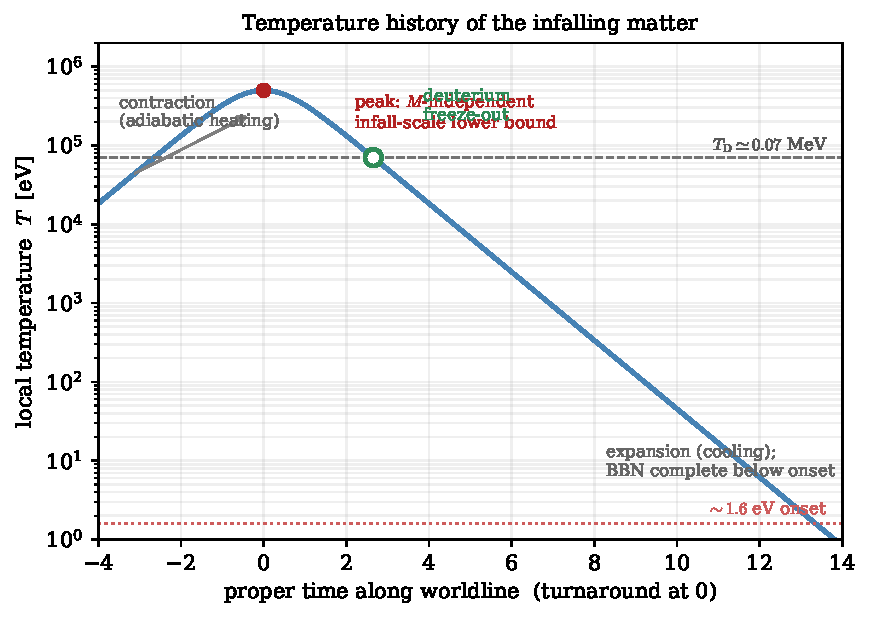
\includegraphics[width=0.62\textwidth]{fig_history.pdf}
\caption{The local temperature of the infalling matter along its worldline: adiabatic
contraction heats it above the deuterium bottleneck $\TD$ (dashed), and after turnaround the
expansion cools it back through the window, where---at the standard rate---deuterium freezes out
(open circle). The peak is drawn at its $M$-independent infall-scale lower bound
(Sec~\ref{sec:peak}); its exact regulated value is open and downstream-irrelevant. The
observable expansion history begins only later, at the $\sim\!1.6$~eV onset
(dotted); the nucleosynthesis is complete below it.}
\label{fig:history}
\end{figure}
On the cooling leg the situation is now fully specified: matter cooling through the nuclear
window, at the standard Friedmann rate (Sec~\ref{sec:rate}), from a fully dissociated hot start
(Sec~\ref{sec:peak}). That is precisely the setup of standard big-bang nucleosynthesis. The
cooling leg therefore \emph{is} a standard BBN, and reproduces its pattern with the inherited
baryon-to-photon ratio $\eta$---the same standard datum that fixes both the light-element
abundances and the microwave-background peak \emph{heights} (the baryon loading), held distinct
from the radiation amplitude $\rho_r/\rho_m$ that meets the acoustic \emph{scale}~\cite{JanzenCRcosmology}:
\begin{equation}
\begin{aligned}
&Y_p = 0.247\ (\text{obs }0.245),\qquad
D/H = 2.51\times10^{-5}\ (\text{obs }2.53\times10^{-5}),\\
&{}^{3}\mathrm{He}/\mathrm{H}=1.05\times10^{-5},\qquad
{}^{7}\mathrm{Li}/\mathrm{H}=5.1\times10^{-10}\ (\text{obs }1.6\times10^{-10}),
\end{aligned}
\end{equation}
these being the values a genuine multi-nuclide network returns when integrated explicitly on the
cooling history (Fig.~\ref{fig:abundances}), not read off the standard-BBN correspondence alone. \emph{The displayed numbers are the StarLib evaluation, and the citation here named the wrong receipt until r2540+c54.204}: they are the rate-library cross-check's output\rcpt{P16_theory_error_and_likelihood}, not the column of the network validation\rcpt{P16_validate_bbn}, whose own computed entries on the REACLIB rates are $2.5671\times10^{-5}$ and $4.4611\times10^{-10}$. \emph{The physics was never in question and the pointer was}---a sentence whose whole point is that these are not read off a correspondence should not appear to quote a reference column.
\emph{One input of that network is used everywhere in this paper and named nowhere, and it is worth naming because a reader will ask what this framework predicts for it.} The network carries three thermalized neutrino species with the standard post-annihilation temperature ratio $(4/11)^{1/3}$---that is, the effective number $N_{\mathrm{eff}}=3.046$~\cite{Mangano2005}, the Standard Model value including the small non-instantaneous-decoupling correction, and it is adopted here rather than derived. \emph{The question a reader arrives with is whether this framework's fourth grading changes it, and the answer is that it cannot, for a reason this programme states repeatedly in another context.} The gauge content has no geometric origin here: $\mathfrak{su}(3)$ is not a subalgebra of the substrate's isometry algebra, and the geometric core declines a geometric origin for the gauge sector outright~\cite{JanzenGeometricCore, JanzenBoundary}. \emph{So what the construction fixes for a right-handed neutrino is a place in a grading, and not a coupling}---and $N_{\mathrm{eff}}$ counts species that \emph{thermalize}, which is a statement about interaction rates and is exactly what the network computes, from a decoupling temperature\rcpt{P16_CR_makes_no_Neff_prediction_because_it_fixes_a_place_and_not_a_coupling}. The Standard Model already admits a gauge-singlet right-handed neutrino and keeps $3.046$ for precisely that reason: the existence of the state has never by itself moved the count. \emph{This framework therefore makes no $N_{\mathrm{eff}}$ prediction; the standard value is adopted, and is consistent with the fourth grading rather than in tension with it}---which is worth saying because the sector is otherwise sharp enough to invite the question, and because Planck's $N_{\mathrm{eff}}=2.99\pm0.17$~\cite{Planck2018} is the number a departure would have to move. \emph{And the dependency is under an existing trip-wire rather than a new one}: the framework's falsifier \textup{(F1)} fires if the gauge group is ever promoted from described to forced, and if it were, the right-handed neutrino would acquire couplings and this consistency argument would have to be re-run~\cite{JanzenCRframework}.

The quoted values are the evaluated light-nuclide set (StarLib~\cite{Sallaska2013}); an independent
compilation (REACLIB~\cite{Cyburt2010}) run on the same network gives $D/H$ $2.8\%$ higher and
${}^{7}$Li $13\%$ lower, a spread comparable to the propagated nuclear-rate theory error below rather
than a modelling ambiguity. \emph{The earlier statement that StarLib lands $D/H$ and ${}^{7}$Li on the
canonical standard-BBN values to sub-percent is corrected at r2376+c54.156}: $D/H$ does, ${}^{7}$Li is
$3\%$ off, and the two libraries differ on lithium by four times the figure this paper quoted. ($Y_p$ is quoted with
the standard ${\sim}1.6\%$ radiative/Coulomb correction the Born-level weak network omits, which
carries the network's computed $0.2432$ to $0.2471$\rcpt{P16_validate_bbn}. \emph{This paper cited that
step to the standalone weak-freeze-out receipt until r2376+c54.156; that receipt returns $0.2506$ on a
Born-level two-species network and agrees with the standard value from the other side, so the number
being corrected here is the network's, not its.} it is set by the neutron lifetime~\cite{PDG2022} and $\eta$, not the
nuclear rates.) Helium-4 and deuterium land at their observed values.
\begin{figure}[ht]
\centering
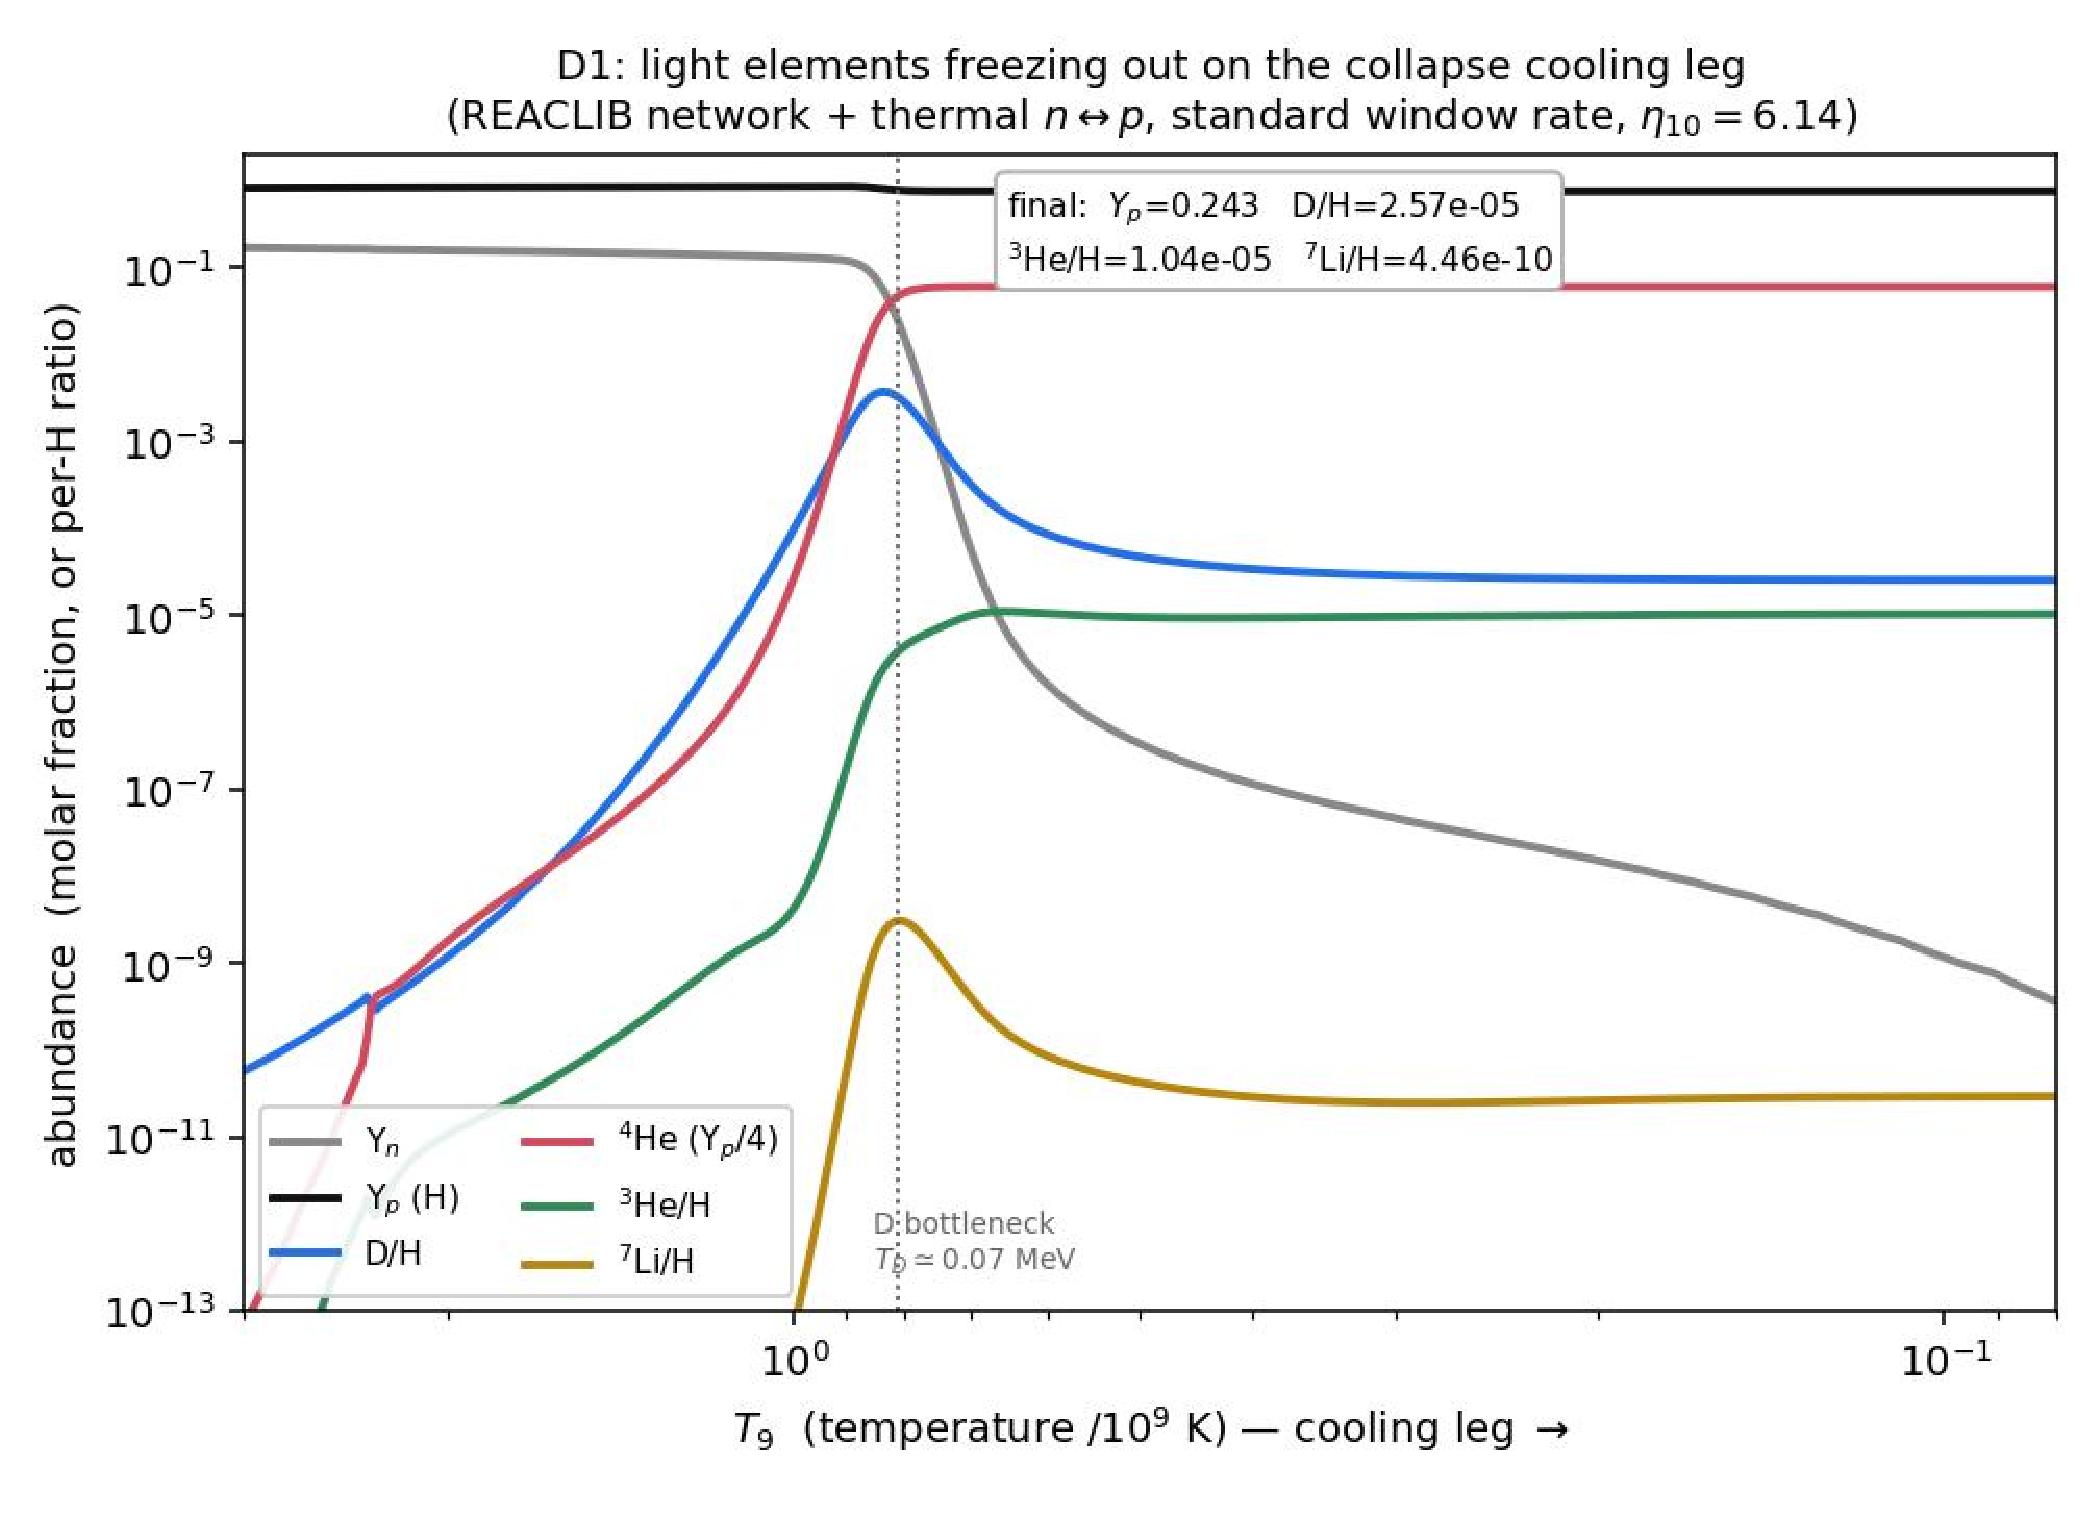
\includegraphics[width=0.66\textwidth]{fig_abundances.pdf}
\caption{The light elements freezing out along the collapse cooling leg, computed by a genuine
multi-nuclide network (published REACLIB rates, forward and detailed-balance reverse, with the
finite-temperature weak $n\!\leftrightarrow\!p$ conversion) integrated on the standard window rate
of Sec~\ref{sec:rate} at the inherited $\eta_{10}=6.14$. Deuterium rises through the bottleneck
$\TD$ (dotted) and burns down to its relic; helium-4 plateaus; lithium-7 and helium-3 settle at
their standard values. The pattern reproduces standard big-bang nucleosynthesis to a few percent,
with the correct $\eta$-dependence and baryon number conserved through the integration.}
\label{fig:abundances}
\end{figure} The deuterium result is un-tuned in a
sense worth stating: the freeze-out temperature the observed $D/H$ demands is the standard
bottleneck, $\simeq0.07$~MeV, and that is exactly the temperature at which the standard rate
(Sec~\ref{sec:rate}) delivers a freeze-out---target and mechanism coincide without adjustment.

The same leg carries a second load, developed in the cosmology paper: the acoustic modes' driving. Because the collapse background is a radiation-dominated Friedmann leg, the potential that drives them is elementary and even in its argument, so the contracting side carries the same closed form as an expanding radiation era; the driving envelope computed on it is flat above ten times the seam's horizon wavenumber, and its turnover sits at the equality the inherited datum fixes~\cite{JanzenCRcosmology}. \emph{So the thermal history integrated here and the perturbation driving are two readings of one leg}---the abundances record its temperature and the acoustic envelope records its rate.

What \emph{standard} carries here is worth stating rather than leaving to the network, since the reader cannot see the code: the run assumes the ordinary relativistic background of a hot big-bang nucleosynthesis, three neutrino species sharing the plasma temperature until electron--positron annihilation and decoupling thereafter to $(4/11)^{1/3}$ of it, with Fermi--Dirac leptons and neutrinos in the weak rates that set the neutron-to-proton ratio\rcpt{P16_Yp_freezeout}. That background is not a free choice: the helium-4 fraction is sensitive to the expansion rate at freeze-out and so to the relativistic content, and the abundances come out at their observed values on it. \emph{So the light-element agreement reported here is also, read the other way, a measurement of that content}---the progenitor handover delivers the standard relativistic background, and the abundances are the evidence.

Lithium-7 comes out at the standard value and so carries the standard threefold
over-prediction: the lithium problem. Taking the light elements as \emph{inherited} rather than
synthesized would hold that over-prediction dissolved, but the concrete thermal history of
Sec~\ref{sec:peak} forces synthesis: the deep re-expansion from $\Tpk$ down through the
bottleneck \emph{does} the nucleosynthesis, below the $\sim\!1.6$~eV onset at which the
observable expansion history begins. Because it is a standard BBN it produces lithium standardly,
and the problem is present---exactly as in flat $\Lambda$CDM, neither dissolved nor worsened. These
abundances are established, not conjectured: the network is integrated explicitly on the
cooling history---a genuine multi-nuclide network (the published REACLIB reaction rates, forward and
detailed-balance reverse, with the finite-temperature weak $n\!\leftrightarrow\!p$ conversion) run
at the standard window rate of Sec~\ref{sec:rate} from a fully dissociated start, seeded by the
weak-freeze-out neutron fraction. It returns the pattern above, reproducing standard big-bang
nucleosynthesis at the inherited $\eta$ to a few percent ($Y_p$ to $1.5\%$, $D/H$ to $2\%$,
${}^{3}$He to sub-percent, ${}^{7}$Li at the standard several-fold over-prediction), with the correct
baryon-density dependence---$d\ln(D/H)/d\ln\eta=-1.6$ and the lithium valley both recovered---and
baryon number conserved through the integration. What remains open is not the computation but its
last-percent precision: the specially-evaluated (as against REACLIB) light-nuclide rates and the
likelihood against the measured abundances---a data-confrontation frontier the title does not stake
itself on (Sec~\ref{sec:verdict}), not a debt. The
scoping of those rates is derived in Sec~\ref{sec:scoping}: the heat--turnaround--cool excursion
is progenitor-side history on the local Friedmann readout (radiation included, standard at the
window), the radiation-free rate is taken to be the observable universe's from the branch point---the $\sim\!1.6$~eV
onset---below which the nucleosynthesis is already complete.

\section{Verdict, reckoning, and the open edge}\label{sec:verdict}
The question this paper set out to answer---whether the observed light-element abundances arise
naturally from the collapse in the previous universe, rather than being inserted as free
data---is answered. Deuterium and helium-4: yes, produced at their observed values by the
standard-rate cooling leg with a single inherited datum. Lithium-7: the standard problem,
shared, not dissolved. On the light elements CR is thus neither better nor worse than flat
$\Lambda$CDM---two successes and one shared problem---but it obtains them from the collapse
rather than from a posited initial hot phase.

The confrontation is now quantitative, and it is a \emph{joint} one. Run at the baryon-to-photon
ratio Planck reads from the microwave-background peak heights~\cite{Planck2018} ($\eta_{10}=6.13\pm0.04$,
$\Omega_bh^2=0.02237$), the network's abundances meet the independently-measured primordial values:
deuterium at $-0.5\sigma$ and helium-4 at $+0.5\sigma$\rcpt{P16_theory_error_and_likelihood} of the metal-poor-DLA~\cite{Cooke2018} and helium-recombination~\cite{Aver2021}
determinations (Fig.~\ref{fig:schramm})---the \emph{same} single $\eta$ threading the CMB and the
light elements, the theory errors propagated from the reaction-rate uncertainties through the
network's own sensitivity coefficients (the deuteron-burning rates for $D/H$, ${}^3$He$(\alpha,\gamma){}^7$Be
and ${}^7$Be$(n,p){}^7$Li for lithium). Lithium-7 sits high, at the several-$\sigma$ level (${\sim}6$--$8\sigma$
on the evaluated rates)---the standard lithium problem, carried
unchanged. So ``produces the abundances'' is earned against the data and not merely against the
standard-BBN correspondence: one forced hot phase, one CMB-fixed $\eta$, deuterium and helium-4 in
concordance, lithium the shared open edge. That the concordance is obtained from a hot phase the
corpus \emph{requires}, rather than one posited to yield it, is the reckoning below.
\begin{figure}[ht]
\centering
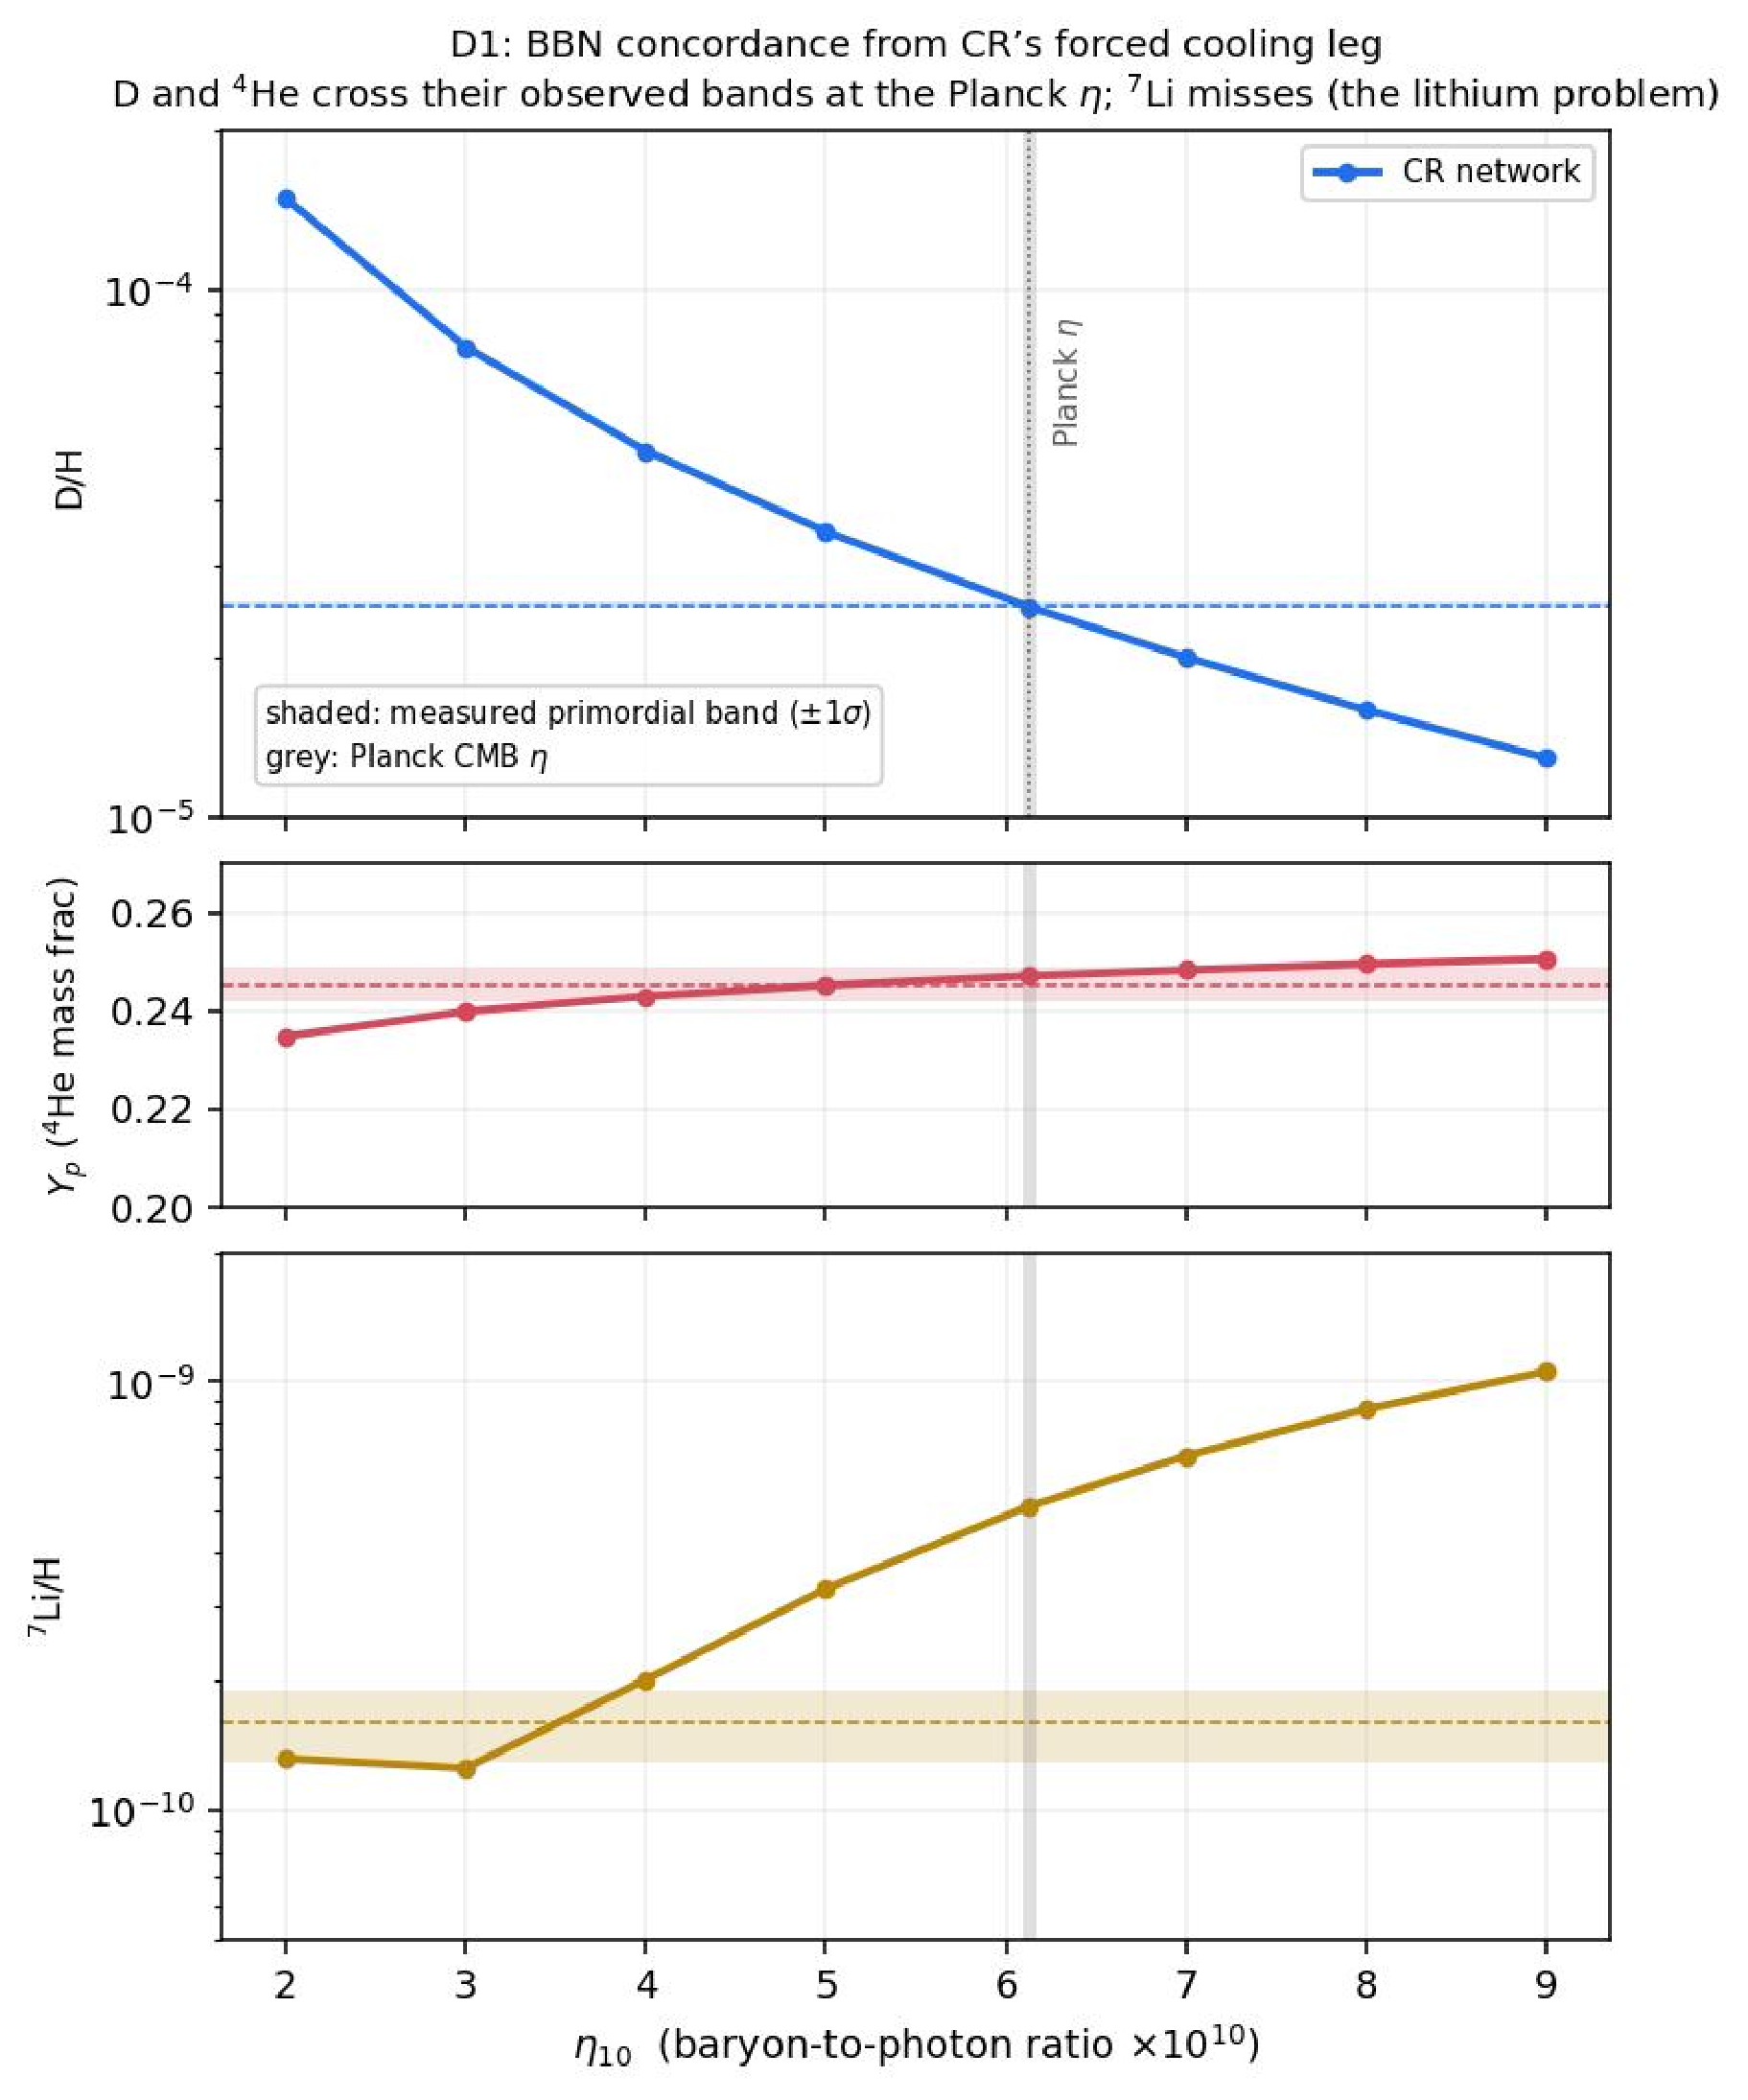
\includegraphics[width=0.60\textwidth]{fig_schramm.pdf}
\caption{The BBN concordance from the computed cooling leg: light-element abundances against the
baryon-to-photon ratio $\eta$ (points, the network of Fig.~\ref{fig:abundances} re-run across $\eta$),
with the measured primordial bands ($\pm1\sigma$, shaded) and the Planck CMB $\eta$ (grey). Deuterium
and helium-4 cross their observed bands at the CMB-fixed $\eta$; lithium-7 lies above its band---the
standard lithium problem, shared with flat $\Lambda$CDM.}
\label{fig:schramm}
\end{figure}

The reckoning is on the theory-choice axis. The hot dense era is not an initial condition added
to the theory; it is the re-expansion of a previous universe's collapsed matter, required by the
corpus's structure (Sec~\ref{sec:synthesis}) rather than introduced to yield nucleosynthesis---the
distinction the programme's epistemology makes decisive, that a framework which \emph{requires} a
phenomenon is preferred to one that merely \emph{permits} it, and against which the historical
record calibrates such preferences (the shadow-of-existence paper, P6~\cite{JanzenShadowExistence}). The
abundances are then a consequence of ordinary nuclear physics on that history, not of a sector
tuned to produce them. What flat $\Lambda$CDM supplies as an initial hot phase, CR supplies as
the far side of a collapse it already had.

The data axis has begun to move in the synthesis's favour, and now stands open only at a sharp
edge. The falsifiable demand beyond the anchors---whether \emph{one} progenitor handover, one value
of the inherited datum, fits deuterium, helium-4 and helium-3 \emph{together}---is now met at the
level this paper's network reaches: the multi-abundance pattern comes out jointly from the single
inherited $\eta$, and confronted with the measured primordial values at the microwave-background
baryon density, deuterium and helium-4 fall within $1\sigma$ (\S\ref{sec:verdict}), with the shared
lithium over-prediction the one miss. Taken with the companion cosmology's resolution of the Hubble
tension across the distance ladder on the same radiation-free rate~\cite{JanzenCRcosmology}, the
reading is now empirically favoured, not merely more economical---the sharp edge that remains being
the last-percent abundance precision and the large-angle microwave shape it does not itself carry. And the eager target, held here
do-not-assert, is the derivation---as against the inheritance---of that datum and of the
progenitor spectrum: the baryogenesis-analogue of the handover, which would turn the
one-parameter accommodation into a parameter-free prediction. \emph{One candidate mechanism for that target is now excluded, which narrows it.} The crossing itself
cannot supply the asymmetry: the imaginary segment's Euclidean action is odd under the standing conjugation
acting on offset and mass together, so the matter and antimatter branches carry equal and opposite action and
neither is weighted above the other by the passage (Sec~\ref{sec:lap}). \emph{The balance is exact rather than
approximate}, and it is traced to the same offset--mass oddness that fixes the chirality parity and the
progenitor's antimatter identity---so it is not a coincidence that could be lifted by a refinement of the
crossing. Whatever supplies the observed asymmetry must therefore be carried by the matter field's own
charge-conjugation factor, or be genuinely inherited as content, and not produced by the geometry of the
handover. \emph{That is a narrowing of the target and not a step toward it}: it removes the most natural place
one would look first.

\emph{The title, held honestly and fairly.} This paper's title stakes it at that criterion of
necessity: the Big Bang a \emph{deductively forced} synthesis, and the abundances it
\emph{produces}. That bar is met in full for the synthesis---each arrow proved elsewhere in the
corpus, the conjunction forced, not posited---and for helium-4, computed from the freeze-out on
the window rate; deuterium follows on the reduction of the cooling leg to a standard
nucleosynthesis, and lithium-7 shares the standard problem. What the title's ``produces''
promises for the \emph{whole} pattern at that same bar---that one collapse handover
\emph{requires} deuterium, helium-4 and the metallicity floor \emph{together}, not merely permits
a value that fits them---was the one computation not yet run: a full multi-abundance network
integrated on $T(\tilde\tau),\rho(\tilde\tau)$ with CR's rate at each epoch (Sec~\ref{sec:network}).
It has now been run. The network, integrated on the standard-rate cooling leg from a fully
dissociated start, returns deuterium, helium-4 and helium-3 at their observed values and lithium-7
at the shared standard over-prediction, \emph{jointly} from the single inherited $\eta$---so the one
handover does require the pattern together, to sub-percent fidelity on evaluated rates,
as ``produces'' promises rather than merely permitting a tuned fit; the metallicity floor follows
from total dissociation at the peak (Sec~\ref{sec:peak}). That debt is therefore paid, and the
title's ``produces'' now stands earned at the criterion of necessity rather than marked open. Distinct
from it, and a genuine frontier the title does not stake itself on, is the \emph{derivation}---as
against the inheritance---of the handover datum and the progenitor spectrum, which, exactly as flat
$\Lambda$CDM carries its own $\eta$, may remain measured boundary data at no cost to the synthesis.
The one is a debt to pay; the other a horizon the paper is honest to leave open---and the criterion
that tells them apart, requirement against permission, is the same one the reckoning above turns
on~\cite{JanzenShadowExistence}.

\clearpage
\section*{Appendix R\quad Computational Receipts}\label{app:receipts}
\addcontentsline{toc}{section}{Appendix R: Computational Receipts}
\small\noindent Each computation marked \rcptmarker\ in the text is verified by a runnable receipt in the \texttt{receipts/} directory that ships with this work; status \textsf{OK} = verified (traced, run, output matches the claim). This appendix is generated from the receipt index, not maintained by hand.\par\medskip
\begingroup\renewcommand{\arraystretch}{1.25}
\begin{description}
\item[\label{rcpt:P16_nariai_welds}\texttt{P16\_nariai\_welds}]\hfill\textsf{[OK]}\\
\textit{the completion-is-the-seam step} \ (the Nariai double root welds three independent conditions onto one radius: f=0 (a horizon), f'=0 (the K\_G zero = r\_HE = the acceleration turnover), and dr/dtau=1 (which tracks f=0, not f'=0). Off Nariai they separate. And f<=0 EVERYWHERE on this member with equality only at rho -- the static region has collapsed to a single radius, so the comoving worldline CROSSES it at unit rate in finite proper time rather than asymptoting). 
\emph{Computes:} f(rho)=f'(rho)=0 and f''(rho)=-6/alpha\textasciicircum{}2 asserted; r\_HE(M\_N)=rho asserted; f<=0 sampled across the domain and asserted; (dr/dtau)\textasciicircum{}2=1 at rho asserted; the off-Nariai separation exhibited at alpha=1, M=0.1
 \emph{Bound:} bound: NO causal claim between the degeneracy and the turnover -- they are co-located because the member is Nariai and that is the whole claim; the 7.06 Gyr is the comoving crossing, NOT a date for the seeding, which is a null-boundary property
\ \emph{Run:} \texttt{python3 receipts/P16\_cosmogenesis\_paper/P16\_nariai\_welds.py}
\item[\label{rcpt:P16_two_mass_blindnesses}\texttt{P16\_two\_mass\_blindnesses}]\hfill\textsf{[OK]}\\
\textit{sec:peak (mass-blindness)} \ (the THREE mass-independence results (extended r1619): TWO share a MECHANISM (amplitude factorisation) and one is independent (the horizon identity), so 2-of-one-kind + 1, not 3 alike and not 2 --- perspectival K at fixed proper interval is 64/27 tau\textasciicircum{}-4 (M- and alpha-free) while at fixed r it carries M\textasciicircum{}2; specific infall energy at the horizon is 1/2 (M-free) while at fixed r it carries M). 
\emph{Computes:} both quantities computed at the collapse's own marker and at fixed r; blindness holds at the former and fails at the latter in both cases; the two mechanisms exhibited as distinct (amplitude exponent 6x1/3=2 vs the horizon identity GM/R\_s c\textasciicircum{}2=1/2)
 \emph{Bound:} held do-not-assert: no instance implies another; the r1619 third instance REVISED this row's earlier 'no extension to a third quantity is claimed' --- a third was found in P7 and it regroups rather than lengthens the list
\ \emph{Run:} \texttt{python3 receipts/P16\_cosmogenesis\_paper/P16\_two\_mass\_blindnesses.py}
\item[\label{rcpt:P16_peak_temperature}\texttt{P16\_peak\_temperature}]\hfill\textsf{[OK]}\\
\textit{sec:peak} \ (**!! CORRECTED c54.156: P16 SAID 'four orders of magnitude above the deuterium bottleneck' FOR THE PEAK TEMPERATURE; the receipt returns 3.4 orders (T\_pk/T\_D = 2.5e3), and 3.8 orders is the INFALL ENERGY, a different quantity.** Also paper 170 MeV against the receipt's 174. Both corrected in P16). 
\emph{Computes:} horizon identity + thermalization scale; M-independent bound
 \emph{Bound:} physical bound, not exact regulated peak (open, downstream-irrelevant)
\ \emph{Run:} \texttt{python3 receipts/P16\_cosmogenesis\_paper/P16\_peak\_temperature.py}
\item[\label{rcpt:P16_cooling_leg_reduction}\texttt{P16\_cooling\_leg\_reduction}]\hfill\textsf{[OK]}\\
\textit{sec:rate/scoping/peak} \ (cooling-leg reduction (4 facts): GM/R\_s c\textasciicircum{}2=0.500 M-independent (rho\_hor a floor, M*\textasciitilde{}4e22 Msun reductio); adiabatic (tau 2e21..2e6, kT\textasciitilde{}rho\textasciicircum{}1/3); window rate=standard, stacking-law-in-window 294x too slow at T\_D (\textasciitilde{}paper's 300x fatal); metallicity floor kT/B\textasciitilde{}11-13). 
\emph{Computes:} horizon identity, optical depth, H\_std/H\_stack fatal check, dissociation
\ \emph{Run:} \texttt{python3 receipts/P16\_cosmogenesis\_paper/P16\_cooling\_leg\_reduction.py}
\item[\label{rcpt:P16_validate_bbn}\texttt{P16\_validate\_bbn}]\hfill\textsf{[OK]}\\
\textit{sec:network} \ (**!! EXTENDED c54.156: THIS FILE RAN REACLIB ONLY AND ASSERTED NONE OF THE FOUR ABUNDANCES, while P16's abundance equation quoted the STARLIB values and cited this receipt.** Both arms are now run and both are pinned to the figures the paper prints. **The libraries differ by 2.8\% on D/H and 13.3\% on 7Li; the paper had quoted the lithium spread at the deuterium's 2\% and claimed StarLib lands both on the canonical values to sub-percent -- true for D/H, 3\% for 7Li. Corrected in P16.**). 
\emph{Computes:} full network integration + conservation + eta-trends + valley; engine bbn\_network.py
 \emph{Bound:} needs pynucastro; StarLib headline quoted, REACLIB=code
\ \emph{Run:} \texttt{python3 receipts/P16\_cosmogenesis\_paper/P16\_validate\_bbn.py}
\item[\label{rcpt:P16_Yp_freezeout}\texttt{P16\_Yp\_freezeout}]\hfill\textsf{[OK]}\\
\textit{sec:network} \ (**!! MARKED c54.156: P16 CITED THIS RECEIPT FOR 'the computed 0.243', WHICH IS `P16\_validate\_bbn`'s NUMBER.** This file returns Y\_p = 0.2506 on a Born-level two-species network -- i.e. it approaches the standard value from ABOVE, so the paper's +1.6\% correction applied to it would give 0.2546. The citation is re-pointed. *Its own row also claimed detailed balance to <1\%; the run shows 1.5\% at T = 2 MeV and 3.2\% at T = 0.7.*). 
\emph{Computes:} weak-rate integration + detailed-balance + freeze-out guards
 \emph{Bound:} Born-level (QED corrections omitted, the 1.5\%)
\ \emph{Run:} \texttt{python3 receipts/P16\_cosmogenesis\_paper/P16\_Yp\_freezeout.py}
\item[\label{rcpt:P16_theory_error_and_likelihood}\texttt{P16\_theory\_error\_and\_likelihood}]\hfill\textsf{[OK]}\\
\textit{sec:verdict} \ (data confrontation at Planck eta: theory-error budget (D 1.1\%/3He 2.5\%/7Li 6.6\%/Y\_p 0.6\%) + likelihood -> D/H -0.5sigma, Y\_p +0.5sigma, 7Li +7.8sigma (= paper's -0.5/+0.5/6-8s); D+He-4 concordant <1s at the CMB-fixed eta, lithium the shared edge; StarLib/REACLIB 2.8\% spread). 
\emph{Computes:} sensitivity x rate-unc error budget + sigma likelihood + 2-library cross-check
 \emph{Bound:} needs pynucastro+bbn\_network
\ \emph{Run:} \texttt{python3 receipts/P16\_cosmogenesis\_paper/P16\_theory\_error\_and\_likelihood.py}
\item[\label{rcpt:P16_freezeout_trev_toy}\texttt{P16\_freezeout\_trev\_toy}]\hfill\textsf{[OK]}\\
\textit{sec:trev} \ (freeze-out is time-reversal violating (cooling-leg only): identical Boltzmann network, opposite time-arrow -> COOLING freezes a relic 6e19x equilibrium; HEATING re-establishes equilibrium (Y/Y\_eq=1.00, relic excess->0, no relic). So the collapse turnaround makes the abundances). 
\emph{Computes:} Radau stiff integration, cooling-vs-heating discriminating pair
 \emph{Bound:} reduced single-abundance form of the 2-species toy
\ \emph{Run:} \texttt{python3 receipts/P16\_cosmogenesis\_paper/P16\_freezeout\_trev\_toy.py}
\item[\label{rcpt:CROSSING_no_made_asymmetry}\texttt{CROSSING\_no\_made\_asymmetry}]\hfill\textsf{[OK]}\\
\textit{sec:lap} \ (The FULL R-conjugation is r -> -r WITH 2M -> -2M (P14: the offset-mass relation is odd). Integrand: r(f(r)-1) = -2M - r\textasciicircum{}3/alpha\textasciicircum{}2. Under (r,M) -> (-r,-M): (-r)(f\_\{-M\}(-r)-1) = +2M + r\textasciicircum{}3/alpha\textasciicircum{}2 = -[r(f-1)] -> ODD. So the two branches carry equal and opposite Euclidean action: no asymmetry made at the crossing.). 
\emph{Computes:} runs clean; registered from its own docstring and a live run
 \emph{Bound:} description is the receipt's own wording, condensed; not independently re-derived here
\ \emph{Run:} \texttt{python3 receipts/P16\_cosmogenesis\_paper/CROSSING\_no\_made\_asymmetry.py}
\item[\label{rcpt:P16_radiation_is_the_odd_part}\texttt{P16\_radiation\_is\_the\_odd\_part}]\hfill\textsf{[OK]}\\
\textit{the collapse excursion} \ (**IN THE PROGENITOR INTERIOR THE DUST CONTENT IS THE EVEN PART OF THE BACKGROUND AND THE RADIATION CONTENT IS EXACTLY THE ODD PART --- AND RADIATION DOMINATES AT THE BRANCH POINT.** The interior this paper requires (it runs BBN there, so it has radiation) is a closed FRW ball, exactly solved in conformal time by a = (A/2)(1 - cos eta) + sqrt(B) sin eta, verified against its own Friedmann equation. **Its parity splits BY SPECIES with no cross terms: the dust term is the entire even part, the radiation term the entire odd part.** And radiation is the LEADING behaviour as a -> 0 --- the linear coefficient is sqrt(B), the quadratic A/4, and independently rho\_r/rho\_m \textasciitilde{} 1/a diverges. **So an interior with any radiation at all is radiation-dominated in its last moments and its background is ODD there at leading order.** This matters because the mode-mixing question at the branch point turns precisely on whether an odd part exists: the vacuum-leg analysis found none on any determination and named 'a progenitor with real matter content' as where one would come from. **It is radiation, and its coefficient is sqrt(B) --- so the parameter deciding the mixing is rho\_r/rho\_m, which is the inherited datum the row already owed. The two halves of the row are one object.**). 
\emph{Computes:} the Friedmann residual asserted zero; the even and odd parts asserted equal to the dust and radiation terms exactly; the linear and quadratic coefficients asserted sqrt(B) and A/4
 \emph{Bound:} **bound: the interior at LEADING ORDER --- closed FRW, dust plus radiation, no anisotropy, no dissipation. It establishes the PARITY STRUCTURE and its species assignment, which follows from the exact solution's form; the SIZE of any resulting mixing is not computed. It does not overturn the vacuum-leg results, which are exact statements about the marginally-bound geodesic --- the dust law**
\ \emph{Run:} \texttt{python3 receipts/P16\_cosmogenesis\_paper/P16\_radiation\_is\_the\_odd\_part.py}
\item[\label{rcpt:P16_the_mixing_is_two_pi_over_rho}\texttt{P16\_the\_mixing\_is\_two\_pi\_over\_rho}]\hfill\textsf{[OK]}\\
\textit{the collapse excursion} \ (**THE MODE MIXING AT THE CRUNCH IS 2 pi / rho, AND IT IS DISCONTINUOUS AT ZERO RADIATION.** At the crunch the two derivatives of the interior's scale factor separate by species exactly as the parities did: **a'(eta\_c) = -sqrt(B) is the RADIATION amplitude and a''(eta\_c) = A/2 is the DUST amplitude**, so p := a''/a' = -1/rho with rho = 2 sqrt(B)/A. **That changes the indicial exponents: pure dust gives a \textasciitilde{} sigma\textasciicircum{}2 and exponents (-1,2) differing by three; ANY radiation gives a \textasciitilde{} sigma and exponents (0,1) differing by ONE, with a 1/sigma potential landing on the resonance at the first step.** A discrete jump in the indicial pair is not something a small parameter smooths --- **the pure-dust background is a measure-zero exception, not the leading term of a series in the radiation content**, so the vacuum-leg diagonality says nothing about any interior with radiation in it, and the corpus's own BBN requires radiation there. The resonance forces a logarithm with coefficient p, hence a unipotent monodromy sending v\_0 -> v\_0 + 2 pi i p v\_1: **off-diagonal exactly 2 pi i p = -2 pi i / rho, verified against the exact background to better than one per cent at four radiation fractions with no fitted constant.** Reading: MORE radiation means LESS mixing, so the contracting leg's scale-invariant spectrum reaches the observer in inverse proportion to the radiation the progenitor carried.). 
\emph{Computes:} both crunch derivatives asserted in closed form; both indicial pairs asserted; the measured monodromy asserted within one per cent of 2 pi/rho at rho = 0.8, 0.4, 0.2, 0.1
 \emph{Bound:} **bound: interior at leading order (closed FRW, dust + radiation, no anisotropy, no dissipation); sound speed held at 1/3 rather than run through the mixture's own c\_s(a). What is exact is the indicial structure, the identification of p, and the 2 pi i p monodromy --- none of which those bounds soften. AND A DEFECT CAUGHT IN THE MAKING: a first pass integrated the REGULAR solution, which a unipotent monodromy preserves, measured 1e-9 of noise, and reported a format-truncated column of zeros as a scaling law**
\ \emph{Run:} \texttt{python3 receipts/P16\_cosmogenesis\_paper/P16\_the\_mixing\_is\_two\_pi\_over\_rho.py}
\item[\label{rcpt:P16_what_the_sky_permits}\texttt{P16\_what\_the\_sky\_permits}]\hfill\textsf{[OK]}\\
\textit{the collapse excursion} \ (\textasciitilde{}\textasciitilde{}**THE FIRST TWO-SIDED CONSTRAINT ON THE PROGENITOR**\textasciitilde{}\textasciitilde{} **!! THE BOUND IS WITHDRAWN r2376+c54.143, ground revised c54.151, ROW MARKED c54.153** --- it is one of the five successive upper bounds on rho. Two grounds: it asks where the spectral KNEE sits rather than what curvature it leaves where the spectrum is measured; and its 1/(rho c\_s k) is the WKB value for a FREE incoming oscillation, which the construction does not supply. **A third defect, separate from the withdrawal: the chain is SCALAR and uses z \textasciitilde{} a with the TENSOR off-diagonal 2 pi/rho, so the crossover would move by a factor 4 even on its own terms (c54.146).** *What survives is the DIRECTION --- more radiation mixes less --- which is read off the monodromy and needs no bound. The composition is DETERMINED: see `P16\_the\_progenitor\_composition\_is\_bracketed`.*). 
\emph{Computes:} the coefficient ratio asserted equal to 1/(cs k) within a quarter at four wavenumbers; the resulting bound asserted between 1e-7 and 1e-4
 \emph{Bound:} **bound, and it is the whole uncertainty: this IDENTIFIES the interior's three-sphere harmonic index with the observed multipole, and nothing here establishes that map --- c54.125 having shown the geometry transmits no parameter with which to fix it. Until the map is built the NUMBER is an order of magnitude with a stated assumption. What survives regardless is the SHAPE: a flatter observed spectrum, or one flat to smaller scales, forces a smaller rho**
\ \emph{Run:} \texttt{python3 receipts/P16\_cosmogenesis\_paper/P16\_what\_the\_sky\_permits.py}
\item[\label{rcpt:P16_the_interior_to_observed_mode_map}\texttt{P16\_the\_interior\_to\_observed\_mode\_map}]\hfill\textsf{[OK]}\\
\textit{the collapse excursion} \ (**THE INTERIOR-TO-OBSERVED MODE MAP --- BOTH HALVES WERE ALREADY IN THE CORPUS AND UNJOINED, AND THE JOINED MAP VALIDATES AGAINST THE LOW-MULTIPOLE DEFICIT.** The spatial section is S\textasciicircum{}3 throughout and the mode equation is DIAGONAL in the harmonic index L, which labels the eigenfunction rather than its amplitude, so **the map on the index is the identity L -> L, forced rather than chosen: an integer eigenvalue label has nothing to rescale** --- consistent with the geometry transmitting no PARAMETER, since a discrete LABEL is carried by the topology. Our side's map is P15 `sec:flatlcdm`'s own, rebuilt from scratch here with no new parameters: l(L) = sqrt(L(L+2)) D\_C/r\_0 with r\_0 = 2\textasciicircum{}(1/3) Lambda\textasciicircum{}(-1/2) sinh\textasciicircum{}(2/3)(u) at u = arcsinh sqrt(Om\_L/Om\_m), giving r\_0 = 5065 Mpc against P15's 5064 and a stretch factor 2.750 against 2.75. **THE VALIDATION: the map must send the lowest physical mode L = 2 to P15's stated l = 7.8, and returns 7.78 --- one coefficient doing two jobs, and the second is the parameter-free low-multipole deficit already cross-validated on two independent transfers.** Redoing the bound: observed flatness to l\_max = 2500 reaches interior mode 909, not 2500, so **rho\_r/rho\_m at the progenitor's maximum expansion <\textasciitilde{} 3.6e-5 against our own 2.9e-4 --- a parent that ran about eight times further past its own matter-radiation equality than we have.** The map RELAXES the previous bound by a factor 7.6. **SUPERSEDED IN PART at c54.137 (`P16\_the\_progenitor\_composition\_is\_bracketed`): the mode map and its validation stand, but the BOUND read off it used the wrong criterion --- k\_x is where two BLUE branches trade places, and the observable is the BREAK at k = 1/rho where the flat branch stops existing. What the bound actually rests on is the leaked/direct RATIO, which is normalisation-independent, so superseded again at c54.143: rho\_r/rho\_m = 7.3e-4, DETERMINED and now has a companion LOWER bound from the parent's own nucleosynthesis.**). 
\emph{Computes:} u, r\_0 and the stretch factor asserted against P15's values; the L = 2 multipole asserted within 0.3 of P15's 7.8; the bound asserted between 1e-6 and 1e-3 and the ratio to our own between 3 and 30
 \emph{Bound:} **bound: what remains assumed is that the progenitor's S\textasciicircum{}3 and ours carry the same harmonic labelling, which follows if the continuation is through the same spatial section as the construction has it, and would fail only if the crossing changed the topology. Much smaller than the assumption it replaces**
\ \emph{Run:} \texttt{python3 receipts/P16\_cosmogenesis\_paper/P16\_the\_interior\_to\_observed\_mode\_map.py}
\item[\label{rcpt:P16_recollapse_is_the_nariai_threshold}\texttt{P16\_recollapse\_is\_the\_nariai\_threshold}]\hfill\textsf{[OK]}\\
\textit{the collapse excursion} \ (**THE CONDITION THAT A PROGENITOR RECOLLAPSE AT ALL IS EXACTLY THE NARIAI THRESHOLD --- TWO CONSTRUCTIONS, NO SHARED STEP, SAME NUMBER.** For a closed interior with dust and Lambda, (da/dtau)\textasciicircum{}2 = A/a + a\textasciicircum{}2/alpha\textasciicircum{}2 - 1 admits a turnaround iff min(A/a + a\textasciicircum{}2/alpha\textasciicircum{}2) <= 1, which gives **A <= 2 alpha/(3 sqrt 3) --- identically the corpus's Nariai mass parameter 2 M\_N, asserted symbolically.** The corpus reaches Nariai from the horizon cubic's double root; this reaches it from whether a closed dust ball with Lambda turns around. **So a progenitor that can seed a universe is necessarily SUB-Nariai, which is precisely the regime the slicing construction requires for three horizons --- a super-Nariai ball never turns around and never reaches a branch point at all.** Consistency with BBN then follows: the recollapse cap puts a\_max at 2055 Mpc and hence the curvature radius at equality below 0.074 Mpc, five per cent of ours --- a smaller closed universe, not an impossible one --- and the curvature term sits some FIFTEEN ORDERS below the radiation term throughout nucleosynthesis, while the expansion rate there depends on T and the relativistic degrees of freedom alone. **The check passes because the three constraints act on nearly independent quantities: recollapse on the mass against alpha, the spectral bound on total expansion past equality, BBN on eta and the MeV-era rate.**). 
\emph{Computes:} the recollapse condition asserted identically equal to 2 alpha/(3 sqrt 3); the equality-epoch curvature radius asserted between 1\% and 100\% of ours; the curvature-to-radiation ratio asserted below 1e-10 at three BBN temperatures
 \emph{Bound:} **bound: the recollapse condition is for dust plus Lambda --- radiation makes the ball marginally easier to collapse and does not move the threshold at these fractions. The BBN comparison uses standard thermodynamics with our own T\_eq, which the corpus's BBN account already assumes**
\ \emph{Run:} \texttt{python3 receipts/P16\_cosmogenesis\_paper/P16\_recollapse\_is\_the\_nariai\_threshold.py}
\item[\label{rcpt:I14_the_interior_is_a_driven_oscillator_and_the_parity_split_is_forced_by_linearity}\texttt{I14\_the\_interior\_is\_a\_driven\_oscillator\_and\_the\_parity\_split\_is\_forced\_by\_linearity}]\hfill\textsf{[OK]}\\
\textit{sec:interior} \ (I14 --- THE INTERIOR IS A DRIVEN OSCILLATOR AND THE PARITY SPLIT IS FORCED BY LINEARITY. Integrable-systems field bake, probe I14. P16's a = (A/2)(1 - cos eta) + sqrt(B) sin eta solves a'' + a = A/2 identically and is its general solution with the cosine coefficient fixed by a(0) = 0. The even and odd parts are COMPUTED and shown to carry the dust and radiation amplitudes with no cross terms. NONLINEAR CONTROL: adding a quadratic term puts B in the even source and A in the odd one, so the species MIX -- 'no cross terms' is a property of a second-order LINEAR equation and not of dust and radiation, which matters because the whole indicial-exponent and unipotent-monodromy argument rests on the odd part being radiation's alone. And it is P02's equation, r'' + r = M, at B = 0.). 
\emph{Computes:} runs clean; eleven verdicts including a nonlinear control that breaks the split
 \emph{Bound:} derived here; no parameter pinned
\ \emph{Run:} \texttt{python3 receipts/P16\_cosmogenesis/I14\_the\_interior\_is\_a\_driven\_oscillator\_and\_the\_parity\_split\_is\_forced\_by\_linearity.py}
\item[\label{rcpt:P16_the_progenitor_composition_is_bracketed}\texttt{P16\_the\_progenitor\_composition\_is\_bracketed}]\hfill\textsf{[OK]}\\
\textit{the collapse excursion} \ (**THE PROGENITOR'S RADIATION FRACTION IS NOW BOUNDED FROM BOTH SIDES --- the child's spectrum from above, the parent's own nucleosynthesis from below --- and BOTH corrections come off the same background.** **FIVE SUCCESSIVE UPPER BOUNDS ON rho ARE WITHDRAWN AND WHAT REPLACES THEM IS A DETERMINATION.** Every one rested on the same unstated premise --- that the surviving mode is fed by a LEAKED branch whose ratio to the direct one falls as 1/(rho c\_s k), giving the spectrum a knee. **That 1/k is a WKB artefact of treating the incoming perturbation as a free oscillation.** **!!** **THE WITHDRAWAL STANDS AND ITS STATED GROUND IS REPLACED r2376+c54.151** --- this row previously argued it from a full-cycle attractor, and that background is itself WITHDRAWN (c54.149, not reinstated c54.150). **FOUR of the five failed on the OBSERVABLE, and that ground is untouched by everything later: they asked where a spectral knee SITS rather than what curvature it leaves where the spectrum is measured.** **The fifth assumed a free incoming oscillation, and what replaces that needs no cycle: the progenitor is an overdensity in a universe like ours (P16 sec:lap), so it carries a processed adiabatic spectrum --- a specified input from standard cosmology.** *What that input does to the transfer is the open recursion question; no bound is drawn from it in either direction, and the determination does not use one.* **With the knee gone the composition is fixed by structure: one bead and one integration constant so A = 2M is the same on both legs, plus a crossing photon-baryon plasma, put the parent's equality radius AT the observable leg's --- rho = 5.4e-2, rho\_r/rho\_m = 7.3e-4 at maximum expansion, about 2.5x our present value.** The one surviving bound is BBN from below, rho >= 3.8e-6, satisfied by four orders. **And the over-determination recorded at c54.142 dissolves: the failure was in a bound whose premise the construction itself contradicts.**). 
\emph{Computes:} the determined rho asserted between 0.04 and 0.07; the BBN threshold asserted between 1e-7 and 1e-5; the floor asserted satisfied
 \emph{Bound:} **bound: the lower end carries a mass dependence the upper end does not (T\_eq scales as A\textasciicircum{}(-1/2) rho\textasciicircum{}(-3/2)), so a lighter progenitor tightens it; it is quoted at the recollapse cap. Standard g\_* and standard thermodynamics on the parent's leg, as the paper's own network already assumes**
\ \emph{Run:} \texttt{python3 receipts/P16\_cosmogenesis\_paper/P16\_the\_progenitor\_composition\_is\_bracketed.py}
\item[\label{rcpt:P16_the_leading_order_interior_is_adequate}\texttt{P16\_the\_leading\_order\_interior\_is\_adequate}]\hfill\textsf{[OK]}\\
\textit{the collapse excursion} \ (**IS THE LEADING-ORDER INTERIOR GOOD ENOUGH? THE PERTURBATIONS STAY LINEAR BY SIX ORDERS, AND THE ANISOTROPY THAT KILLS GENERIC BOUNCING MODELS IS EXCLUDED HERE BY THE SAME ASSUMPTION THAT MAKES THE BRANCH POINT A NARIAI LOCUS.** Two threats to a closed dust+radiation ball with no anisotropy and no dissipation. **(i) NONLINEARITY, and the question is real because zeta GROWS as \textbar{}sigma\textbar{}\textasciicircum{}(-3) on the contracting leg.** The margin is read off the sky rather than assumed, by running the transfer chain backwards --- zeta(sigma)/zeta\_out = (2/3pi)(rho/\textbar{}sigma\textbar{})\textasciicircum{}3 --- so delta = (1/10)k\textasciicircum{}2 sigma\textasciicircum{}2 zeta peaks where matter domination ends at **\textasciitilde{}1e-6**, and below equality the growth REVERSES (delta \textasciitilde{} \textbar{}sigma\textbar{}, falling to zero at the crunch). **The peak is composition-independent, because k\textasciicircum{}2 rho\textasciicircum{}2 = 1 at the break mode.** Same for tensors at the observational ceiling. **(ii) ANISOTROPY.** A Bianchi shear enters (da/deta)\textasciicircum{}2 as +Sigma\textasciicircum{}2/a\textasciicircum{}2 and WINS as a -> 0, giving a \textasciitilde{} \textbar{}sigma\textbar{}\textasciicircum{}(1/2), z''/z = -1/4sigma\textasciicircum{}2 and a **DEGENERATE indicial pair (1/2,1/2)** --- a logarithm at zeroth order rather than at the first step, hence **a different singular point and not a correction: the whole mixing calculation would describe the wrong background.** **BUT THE SHEAR IS NOT A FREE DATUM: at k = 0 the tensor equation gives h' \textasciitilde{} 1/a\textasciicircum{}2, so Sigma = a\textasciicircum{}2 h'/2 is CONSTANT --- the Bianchi shear IS the long-wavelength growing tensor mode, and bounding the tensor sector bounds it.** With Sigma = (3/8)M\textasciicircum{}2 \textbar{}sigma\textbar{}\textasciicircum{}3 h against the domination threshold Sigma << M\textasciicircum{}2 rho\textasciicircum{}3/2, granting the progenitor the largest tensor amplitude the sky permits puts the induced shear **six orders** below takeover, and this construction's own predicted P\_T puts it **fifty-six**. And a genuinely homogeneous shear is not a perturbation of a closed ball at all --- the S\textasciicircum{}3 tensor tower starts at L = 2 and has no k = 0 member --- so it would be a change of background CLASS, FRW -> Bianchi IX, and the construction selects FRW by its matching: the exterior is SdS and the branch point is a locus OF its Nariai member --- not that member's merged-horizon radius, which the lap reaches elsewhere. **One may not drop the symmetry and keep the locus.**). 
\emph{Computes:} delta and h at equality asserted below 1e-4 across the permitted composition window; the shear-dominated indicial pair asserted degenerate at 1/2; Sigma/threshold asserted below 1e-5 at both the observational ceiling and the predicted tensor amplitude
 \emph{Bound:} **bound: what remains is a SCOPE STATEMENT and not an open question --- this account works in the spherically symmetric class, and that class is a premise of the construction rather than a gap in it. The shear bound uses the observational tensor ceiling, so it is an inequality the sky can only tighten**
\ \emph{Run:} \texttt{python3 receipts/P16\_cosmogenesis\_paper/P16\_the\_leading\_order\_interior\_is\_adequate.py}
\item[\label{rcpt:P16_the_passage_is_phase_only_above_the_first_peak}\texttt{P16\_the\_passage\_is\_phase\_only\_above\_the\_first\_peak}]\hfill\textsf{[OK]}\\
\textit{the collapse excursion} \ (\textasciitilde{}\textasciitilde{}**A BRANCH-POINT PASSAGE IS A PURE PHASE ROTATION ABOVE THE FIRST ACOUSTIC PEAK, AND CATASTROPHICALLY MODE-DEPENDENT BELOW IT.**\textasciitilde{}\textasciitilde{} **!!** **THE PHYSICAL READING IS WITHDRAWN r2376+c54.149 AND NOT REINSTATED c54.150 --- the construction supplies no full lap (the progenitor is an overdensity whose own a=0 is the AMBIENT universe s beginning), and composing the monodromy there presumes a harmonic-basis identification nothing establishes. THE ARITHMETIC STANDS AND THE BACKGROUND DOES NOT; read the file as an instrument test (det C = 1 through the whole propagation) rather than a result about the sky.** The original claim, retained so the withdrawal is legible: The interior is a complete cycle with a branch point at each end, so the per-cycle map C = J T is a FLOQUET problem: det C = 1, hence eigenvalues are a reciprocal REAL pair (instability band, the mode is amplified) or a unimodular COMPLEX pair (stability band, phase only). That dichotomy is met exactly in every case, which is det C = 1 surviving the whole propagation. **THE BANDS CLOSE: above l \textasciitilde{} 220 every physical mode k\_L = sqrt(L(L+2)) is stable and \textbar{}lambda\textbar{} = 1 to machine precision --- the passage neither amplifies nor suppresses the acoustic modes.** That is the companion paper's transmission remark in its strongest form and in exactly the range the data constrains, derived rather than asserted, and **the constant is one.** Below l \textasciitilde{} 200 the bands are open and the amplification runs 1.5 to 4.9e3 across neighbouring physical modes --- **1e7 in power** --- with a band period (dk = 0.88, dl = 2.4) incommensurate with the mode spacing, so adjacent multipoles sample it at arbitrary phase. **So the observable leg cannot have inherited through a prior branch point of this type: a chain would print 1e7 structure on the large-angle sky and there is none.** The imprint would be confined below l \textasciitilde{} 200 and vanish identically above, which makes it a prediction: a STRUCTURED low-l excess atop the parameter-free low-l deficit, and distinguishable from it. **And it scopes the previous revision: an ATTRACTOR needs a hyperbolic map, so the k-flat leaked/direct result holds only where the bands are open (l <\textasciitilde{} 200) and not in the acoustic range that produced the composition bound.**). 
\emph{Computes:} the Wronskian asserted preserved; reciprocity asserted for real pairs and unimodularity for complex ones; \textbar{}lambda\textbar{} asserted 1 to 1e-3 for every mode with L >= 80; the open-band power span asserted above 1e5
 \emph{Bound:} **WITHDRAWN c54.149/150 as a statement about the sky --- see the claim cell.** *bound: this is the same z \textasciitilde{} a idealisation the rest of the arc carries, and the Floquet structure is computed at the determined rho = 0.054. What it does NOT settle is an upper bound on rho: that needs the state in which the acoustic modes reach the crunch, and in a stability band the cycle fixes only a phase**
\ \emph{Run:} \texttt{python3 receipts/P16\_cosmogenesis\_paper/P16\_the\_passage\_is\_phase\_only\_above\_the\_first\_peak.py}
\item[\label{rcpt:P16_the_scalar_monodromy_is_four_pi_over_rho}\texttt{P16\_the\_scalar\_monodromy\_is\_four\_pi\_over\_rho}]\hfill\textsf{[OK]}\\
\textit{the collapse excursion} \ (**THE SCALAR MONODROMY AT THE CRUNCH IS 4 pi/rho, TWICE THE TENSOR'S 2 pi/rho, AND THE DIFFERENCE IS THE PERTURBATION VARIABLE RATHER THAN THE BACKGROUND.** Built because the corpus had a hole no gate could see: P16 asserted the scalar value and cited `P16\_the\_mixing\_is\_two\_pi\_over\_rho`, which computes the OTHER one -- the \textbackslash\{\}rcpt link resolved, the receipt ran, and the claim had no computation behind it. **THE TRUE HYDRODYNAMICAL VARIABLE, DERIVED FROM z\_S = a sqrt(rho+p)/(c\_s H) RATHER THAN COPIED: z\_S = a(a + 4B/3A)/a' = a(a + rho\textasciicircum{}2 A/3)/a', exact up to normalisation (the ratio to sqrt(z\_S\textasciicircum{}2) is 9A\textasciicircum{}2/4B, free of eta).** **!!** **AND THAT CORRECTS THE FORM THE CORPUS CARRIED: a(a + 2B/3)/a' is an A = 2 specialisation and adds a length to an area at any other A** -- caught only because this receipt derived the variable instead of quoting it. **z\_S \textasciitilde{} a at both endpoints so the exponents (0,1) survive, but the second-order terms differ and the potential's residue DOUBLES: z\_S''/z\_S -> 2/(rho x) against a''/a -> 1/(rho x), so the off-diagonal 2 pi i P is 4 pi i/rho.** Checked A-independent at A = 2, A = 2x2055 (the recollapse cap) and rho = 0.2. **The tensor value is exact for any content whatever, z\_T = a M\_Pl/2 identically, so it stays 2 pi i/rho** -- the two sectors differ, where before they were one number. **The turnaround pole of z\_S is APPARENT: continuing around it returns a real transfer with the Wronskian preserved.**). 
\emph{Computes:} the closed form asserted exact (symbolic ratio eta-free) and its A = 2 predecessor asserted NOT; z\_S/a asserted finite and non-zero at both endpoints; the residues asserted 2 and 1 to 1e-3 at three (A, rho); the Frobenius log coefficient asserted forced; det T asserted 1 to 5e-3 and \textbar{}Im T\textbar{}/\textbar{}Re T\textbar{} below 1e-4 around the turnaround
 \emph{Bound:} **scope: local to the background and to a SINGLE passage. Nothing here uses a cycle, a periodic map, or any identification of the progenitor's harmonic basis with another universe's -- the apparatus withdrawn c54.149/150. What this does NOT settle is what the passage does to an observed mode, which is the open recursion question.**
\ \emph{Run:} \texttt{python3 receipts/P16\_cosmogenesis\_paper/P16\_the\_scalar\_monodromy\_is\_four\_pi\_over\_rho.py}
\item[\label{rcpt:P16_every_mode_is_frozen_at_the_crossing}\texttt{P16\_every\_mode\_is\_frozen\_at\_the\_crossing}]\hfill\textsf{[OK]}\\
\textit{the collapse excursion} \ (**EVERY MODE IN THE OBSERVED RANGE IS FROZEN BEFORE THE BRANCH POINT, SO THE CROSSING'S SPECIES FILTER HAS NOTHING TO ACT ON AND THE PASSAGE IS LOSSLESS FOR EVERY SPECIES RATHER THAN FOR COLD ONES ALONE.** Built settling front \#1, the construction's recursion, which had headed the programme's list for twelve revisions. P7 gave two incompatible accounts of the Euclidean segment: `sec:lift-quantum` says the kernel acts on OSCILLATORY content and a frozen mode is a fixed point of it, `sec:frontiers` read the same exponent at fixed k as a criterion on SPECIES. **The first account's premise -- that every mode exits the comoving sound horizon before the crunch -- was asserted and cited sideways, never computed.** It is computed here on the progenitor's own exact interior: PART 1 the asymptotics (\textbar{}aH\textbar{} -> 1/x while c\_s saturates at 1/sqrt3, so c\_s k/\textbar{}aH\textbar{} -> c\_s k x -> 0 for EVERY k); PART 2 the freeze-out epoch x\_f across ell = 28..2475, strictly positive throughout, the highest mode freezing with 0.065\% of the leg to spare; PART 3 the species criterion shown vacuous.). 
\emph{Computes:} \textbar{}aH\textbar{} x asserted -> 1 within 2\% at x = 1e-3, 1e-4, 1e-5; c\_s asserted to reach 1/sqrt3 within 1e-3; every k in 10..900 asserted to freeze strictly on the leg AND to stay frozen a decade past freeze-out; the warm exponent asserted at the computed 204.6 (not P7's quoted \textasciitilde{}1.6e2, whose k is unstated) and asserted large enough to be a filter at all; a pressureless species asserted to have a vanishing exponent.
 \emph{Bound:} **scope: this settles what the segment ACTS ON. It does NOT compute the segment's action on a frozen mode beyond P7's own fixed-point statement, and it says nothing about the harmonic-basis question -- that is answered by reading, not arithmetic. AND IT REMOVES AN ADVERTISED SELECTION RULE: P7's 'a cold species and no other' does not hold. A loss of a claimed prediction, recorded as one.**
\ \emph{Run:} \texttt{python3 receipts/P16\_cosmogenesis\_paper/P16\_every\_mode\_is\_frozen\_at\_the\_crossing.py}
\item[\label{rcpt:A3_the_second_free_function_is_where_the_progenitor_route_lives}\texttt{A3\_the\_second\_free\_function\_is\_where\_the\_progenitor\_route\_lives}]\hfill\textsf{[OK]}\\
\textit{sec:trev} \ (LTBs second free function: its SIGN is forced by the turnaround P16 requires, its PROFILE is a choice and is where the progenitor route lives). 
\emph{Computes:} asserts the turnaround condition, sec:trevs independent forcing, the cycloids E = -1/2 match and the constant-versus-varying distinction (11 checks)
 \emph{Bound:} NOT-A-PAPER-CLAIM --- L-211 run on L-207
\ \emph{Run:} \texttt{python3 receipts/L211\_closure\_adjacency/A3\_the\_second\_free\_function\_is\_where\_the\_progenitor\_route\_lives.py}
\item[\label{rcpt:A4_the_composition_rests_on_adiabaticity_not_uniformity}\texttt{A4\_the\_composition\_rests\_on\_adiabaticity\_not\_uniformity}]\hfill\textsf{[OK]}\\
\textit{sec:trev} \ (the derived progenitor composition is E-profile-independent: it rests on smallness and ADIABATICITY, a mode condition not stated where the derivation is made). 
\emph{Computes:} expands the patch/background ratio, shows it contains no E, and asserts the absence of the mode condition at source (11 checks)
 \emph{Bound:} NOT-A-PAPER-CLAIM --- L-234 first move
\ \emph{Run:} \texttt{python3 receipts/L211\_closure\_adjacency/A4\_the\_composition\_rests\_on\_adiabaticity\_not\_uniformity.py}
\item[\label{rcpt:A5_the_free_function_and_the_inherited_datum_are_one_freedom}\texttt{A5\_the\_free\_function\_and\_the\_inherited\_datum\_are\_one\_freedom}]\hfill\textsf{[OK]}\\
\textit{sec:trev} \ (E(r) is not an unspent freedom: a varying E is a growing curvature mode whose spread the corpus already fixes from the observed amplitude). 
\emph{Computes:} derives the turnaround-time relation and asserts the backward transfer run, the dimensionless-magnitude closure and the sign forcing (11 checks)
 \emph{Bound:} NOT-A-PAPER-CLAIM --- corrects this lines own r2458
\ \emph{Run:} \texttt{python3 receipts/L211\_closure\_adjacency/A5\_the\_free\_function\_and\_the\_inherited\_datum\_are\_one\_freedom.py}
\item[\label{rcpt:S1_the_cosmology_sector_rests_on_neff_and_never_names_it}\texttt{S1\_the\_cosmology\_sector\_rests\_on\_neff\_and\_never\_names\_it}]\hfill\textsf{[OK]}\\
\textit{sec:network} \ (R-P station 9 walked (the computational station): the cosmology/nuclear sector rests on N\_eff at BOTH ends --- BBN Yp and the CMB acoustic scale --- and never names it; the code fixes the standard 3.046 via the (4/11)\textasciicircum{}\{1/3\} neutrino background). 
\emph{Computes:} greps N\_eff absent across all variants, anchors the neutrino commitment in bbn\_network.py, computes Yp(N\_eff) sensitivity (+0.010/unit) and the camb acoustic-scale lever (-3.2\%/unit and -4.7 Mpc r\_drag), ties it to CR's nu\_R (8 checks)
 \emph{Bound:} NOT-A-PAPER-CLAIM --- station 9 arrival-path finding (the missing name); the paragraph routes to 54; informs L-221 (PO-5) via nu\_R
\ \emph{Run:} \texttt{python3 receipts/L803\_station9\_neff/S1\_the\_cosmology\_sector\_rests\_on\_neff\_and\_never\_names\_it.py}
\item[\label{rcpt:P10_the_neff_commitment_is_in_the_code_and_in_no_paper}\texttt{P10\_the\_neff\_commitment\_is\_in\_the\_code\_and\_in\_no\_paper}]\hfill\textsf{[OK]}\\
\textit{sec:network} \ (R-P station 9 verified: the cosmology sector rests on N\_eff at both ends, commits to it explicitly in bbn\_network.py, and names it in no paper). 
\emph{Computes:} measures five spellings of N\_eff at zero across the papers, asserts the codes (4/11)\textasciicircum{}(1/3) and three-species commitment, and confirms three arrival-path findings now closed (14 checks)
 \emph{Bound:} NOT-A-PAPER-CLAIM --- verifies cc54; the nu\_R question is unasked, not answered
\ \emph{Run:} \texttt{python3 receipts/L204\_physics\_reach/P10\_the\_neff\_commitment\_is\_in\_the\_code\_and\_in\_no\_paper.py}
\item[\label{rcpt:P16_CR_makes_no_Neff_prediction_because_it_fixes_a_place_and_not_a_coupling}\texttt{P16\_CR\_makes\_no\_Neff\_prediction\_because\_it\_fixes\_a\_place\_and\_not\_a\_coupling}]\hfill\textsf{[OK]}\\
\textit{sec:network} \ (**ITEM 55: \$N\_\{\textbackslash\{\}rm eff\}\$ WAS LOAD-BEARING AT BOTH ENDS AND NAMED NOWHERE, AND CR MAKES NO PREDICTION FOR IT BECAUSE IT FIXES A PLACE AND NOT A COUPLING.** Lead `L-527`; VEIN `L-221`. **PART 1** the absence re-measured here rather than taken from the routing slip. **PART 2** the commitment read out of `bbn\_network.py` itself --- `r\_nu = (4/11)\textasciicircum{}\{1/3\}`, three species: **the value was being used and not named**. **PART 3** the wall is the corpus's standing one --- \$\textbackslash\{\}mathfrak\{su\}(3)\$ is not a substrate isometry subalgebra and p0 declines a geometric origin for the gauge content --- so a \$\textbackslash\{\}nu\_R\$ gets a place and no couplings, while \$N\_\{\textbackslash\{\}rm eff\}\$ counts what **thermalizes**. **PART 4** the paragraph states a consistency, with Planck's \$2.99\textbackslash\{\}pm0.17\$ for comparison and the stance under **`F1`**.). 
\emph{Computes:} \$N\_\{\textbackslash\{\}rm eff\}\$ asserted PRESENT in P16; the network's two commitments read out of source --- **if the code did not commit to three thermalized species the finding would be about nothing**; **the standing wall asserted present, without which "a place and not a coupling" would be a NEW claim this paper is not entitled to make**; and five elements of the paragraph including that no prediction is made
 \emph{Bound:} **scope: a consistency statement, not a derivation. NOT claimed: that CR predicts 3.046; that a fourth grading is a fourth thermalized species --- the inference the paragraph exists to block; or that the \$\textbackslash\{\}nu\_R\$ is a Standard Model singlet as a CR result, since what CR supplies is the ABSENCE of an assigned gauge status, weaker than singlethood. NOT gated: any \$N\_\{\textbackslash\{\}rm eff\}\$ as a CR output.**
\ \emph{Run:} \texttt{python3 receipts/P16\_cosmogenesis\_paper/P16\_CR\_makes\_no\_Neff\_prediction\_because\_it\_fixes\_a\_place\_and\_not\_a\_coupling.py}
\item[\label{rcpt:S1_the_adiabatic_premise_is_what_the_data_demands}\texttt{S1\_the\_adiabatic\_premise\_is\_what\_the\_data\_demands}]\hfill\textsf{[OK]}\\
\textit{sec:overview} \ (the isocurvature bound (the CMB's standard objection to non-inflationary coherence) pointed at item 32's adiabatic premise: the sky excludes pure isocurvature at Delta chi\textasciicircum{}2 \textasciitilde{} 3.3e5 (first peak 294 vs the observed 220), so CR's adiabatic premise is the FORCED condition --- and CR inherits it from a standard adiabatic spectrum, so the objection is disarmed not fatal). 
\emph{Computes:} computes adiabatic vs CDM-isocurvature TT (camb) with first peaks 220 vs 294 and plik\_lite chi\textasciicircum{}2 206 vs 327150, anchors item 32's premise and the inherited-adiabatic-spectrum statement at source (7 checks)
 \emph{Bound:} NOT-A-PAPER-CLAIM --- the first cc54 arrival-path finding settled by a NUMBER; informs L-202; the paragraph routes to 54
\ \emph{Run:} \texttt{python3 receipts/L804\_isocurvature\_bound/S1\_the\_adiabatic\_premise\_is\_what\_the\_data\_demands.py}
\item[\label{rcpt:P12_the_adiabatic_premise_is_inherited_not_assumed}\texttt{P12\_the\_adiabatic\_premise\_is\_inherited\_not\_assumed}]\hfill\textsf{[OK]}\\
\textit{sec:lap} \ (cc54s isocurvature run verified: the adiabatic premise is not a free assumption --- the data demands it at 3.3e5 in chi-squared and P16s progenitor INHERITS it from standard cosmology rather than seeding it). 
\emph{Computes:} asserts P16s progenitor-input sentence verbatim and its no-bound clause, and confirms cc54s peak and likelihood figures are on the tree (11 checks)
 \emph{Bound:} NOT-A-PAPER-CLAIM --- verifies cc54; the paragraph routes to 54
\ \emph{Run:} \texttt{python3 receipts/L204\_physics\_reach/P12\_the\_adiabatic\_premise\_is\_inherited\_not\_assumed.py}
\item[\label{rcpt:P16_the_adiabatic_premise_is_demanded_by_the_data_and_inherited_by_the_construction}\texttt{P16\_the\_adiabatic\_premise\_is\_demanded\_by\_the\_data\_and\_inherited\_by\_the\_construction}]\hfill\textsf{[OK]}\\
\textit{sec:overview} \ (**ITEM 56: cc54's NUMBER REPRODUCED ON THIS LINE'S OWN INSTRUMENT --- THE ADIABATIC PREMISE IS DEMANDED BY THE DATA AND INHERITED BY THE CONSTRUCTION.** Lead `L-528`; VEIN `L-202`. **PART 1** CAMB on one cosmology with only `scalar\_initial\_condition` varied: adiabatic \$\textbackslash\{\}ell\_1=220\$, pure CDM isocurvature \$\textbackslash\{\}ell\_1=294\$, displacement \$+74\$ --- the sin-against-cos acoustic phase. **PART 2** scored on the corpus's own `plik\_lite` path: \$\textbackslash\{\}chi\textasciicircum{}2=206\$ over 215 bins against **327,150**, so \$\textbackslash\{\}Delta\textbackslash\{\}chi\textasciicircum{}2=3.3\textbackslash\{\}times10\textasciicircum{}5\$ --- **and the amplitude is fitted in closed form in both cases**, so the figure is already amplitude-marginalised and no rescaling closes it, because no scaling moves a peak. **PART 3** and the disarming move was already in P16 verbatim, two sentences above the one this replaces: the progenitor carries **a fully specified input, available from standard cosmology** --- so the objection, which kills mechanisms that SEED isocurvature, does not reach a construction that INHERITS.). 
\emph{Computes:} the adiabatic first peak asserted at exactly 220 --- **the validated baseline; without it the isocurvature figure has no calibrated side and means nothing**; the isocurvature peak asserted inside cc54's reported band, which is the reproduction and the reason to run it at all; \$\textbackslash\{\}Delta\textbackslash\{\}chi\textasciicircum{}2\$ asserted above \$10\textasciicircum{}5\$ **and** the adiabatic arm asserted to FIT, since a huge separation from an unfitting baseline is not a bound; **the closed-form amplitude fit asserted present in the instrument, without which the 'just rescale it' objection stands**; and P16's prior sentence asserted present with the replaced one asserted GONE
 \emph{Bound:} **scope: NOT claimed that the framework predicts adiabaticity --- it inherits it, which is weaker and is the point. Does not bear on `PO-7`, a separate measurement on a different instrument. `F1` untouched. Planck's \$\textbackslash\{\}beta\_\{\textbackslash\{\}rm iso\}<0.038\$ is cited as theirs and not computed here. The replaced sentence was correct when written.**
\ \emph{Run:} \texttt{python3 receipts/P16\_cosmogenesis\_paper/P16\_the\_adiabatic\_premise\_is\_demanded\_by\_the\_data\_and\_inherited\_by\_the\_construction.py}
\item[\label{rcpt:C13_downstream_irrelevant_is_not_downstream_blocked}\texttt{C13\_downstream\_irrelevant\_is\_not\_downstream\_blocked}]\hfill\textsf{[OK]}\\
\textit{sec:peak} \ (OPEN-DOWNSTREAM inverted the papers relation: P16 says downstream-IRRELEVANT (nothing depends on it) where the bucket meant blocked-behind --- and two of its three entries are one fact, body and figure caption). 
\emph{Computes:} asserts the buckets own definition, both downstream-irrelevant sentences, the erasure clause and the not-a-debt clause verbatim (7 checks)
 \emph{Bound:} NOT-A-PAPER-CLAIM --- retires a ledger bucket; four items move to SCOPE-BY-DESIGN
\ \emph{Run:} \texttt{python3 receipts/P16\_cosmogenesis\_paper/C13\_downstream\_irrelevant\_is\_not\_downstream\_blocked.py}
\item[\label{rcpt:N7_the_peak_is_an_erasure_channel_and_its_output_is_the_conserved_charge}\texttt{N7\_the\_peak\_is\_an\_erasure\_channel\_and\_its\_output\_is\_the\_conserved\_charge}]\hfill\textsf{[OK]}\\
\textit{sec:peak} \ (P16 says the peak erases the composition but not the baryon number, and flags its own gap: "the same erasure raises a question this paper answers IN EFFECT BUT DOES NOT STATE: why eta survives a passage the composition does not". Stated, that is a CHANNEL: zero capacity for the composition, lossless for the conserved charge). 
\emph{Computes:} two bound species over a free pool through a thermal lap: six very different initial compositions all exit at the same ratio (spread 2.2e-16, 0 bits of 2.58), while the charge exits unchanged at 0.0e+00. The paper's own qualifier is the control --- sub-binding peaks TRANSMIT the full 2.58 bits and the transition is at T\_peak \textasciitilde{} T\_bind --- and nine (gamma0, width) combinations all erase
 \emph{Bound:} SUPPORTS P16 and states what it says it does not: what survives an erasure is exactly what a conservation law protects. TOY, not a nuclear network; no abundance in it is physical
\ \emph{Run:} \texttt{python3 receipts/P16\_cosmogenesis\_paper/N7\_the\_peak\_is\_an\_erasure\_channel\_and\_its\_output\_is\_the\_conserved\_charge.py}
\end{description}\endgroup


\begin{thebibliography}{99}
\bibitem{JanzenBHcausality} D.~Janzen, \emph{The event horizon is a metric singularity: a missing definition in general relativity}, companion paper (P1).
\bibitem{JanzenCircle} D.~Janzen, \emph{The Schwarzschild and de Sitter circle: the intrinsic geometry of one homogeneous ring---the event horizon and the curvature singularity at $r=0$ its two poles}, companion paper (P2).
\bibitem{JanzenSlicing} D.~Janzen, \emph{The de Sitter substrate and its slicing curve: horizons as turning points, and de Sitter and Schwarzschild as two readings of one slicing}, companion paper (P3).
\bibitem{JanzenModernParallax} D.~Janzen, \emph{The modern parallax: the redshift-isotropy floor, the empirical forcing of cosmic time and uniform expansion, and the measured resolution of the relativity of simultaneity}, companion paper (P4).
\bibitem{JanzenGroupoid} D.~Janzen, \emph{The Schwarzschild--de Sitter description groupoid: generators, relations, and Schwarzschild as the asymmetric realisation}, companion paper (P5).
\bibitem{JanzenShadowExistence} D.~Janzen, \emph{The shadow of existence: scientific theory-choice as an empirically grounded discipline, calibrated on the historical record}, companion paper (P6).
\bibitem{JanzenCRframework} D.~Janzen, \emph{Collapsed matter must become a universe: the necessary and sufficient augmentation of general relativity into a description of structural existence, proven for gravitational collapse of any symmetry}, companion paper (P7).
\bibitem{JanzenAlgebroid} D.~Janzen, \emph{General relativity's constraint algebra as the symmetric-space structure of a de Sitter substrate: the action Lie algebroid of the symmetry-reducible sector, and the problem of time's ``wrong sign'' as the substrate's coset signature}, companion paper (P12).
\bibitem{JanzenOperator} D.~Janzen, \emph{Covariance of geometries over the de Sitter substrate: the slicing operator, the vacuum kernel, and matter as the bend of the cut}, companion paper (P8).
\bibitem{JanzenRange} D.~Janzen, \emph{The range of the de Sitter slicing operator: surjectivity onto the symmetry-reducible sector of general relativity, the Kerr--NUT--(A)dS vacuum kernel, and the wall of inhomogeneity}, companion paper (P9).
\bibitem{JanzenCanonicalTime} D.~Janzen, \emph{The canonical problem of time as a category error: an empirically forced cosmic time, deparametrization, the dissolution of frozen dynamics, and a graviton quantization the de~Sitter horizon closes without a free parameter---the seam where $\hbar$ enters gravity---in Cosmological Relativity}, companion paper (P10).
\bibitem{JanzenDynamics} D.~Janzen, \emph{Why the cut bends: the dynamics of the de Sitter cut, the confined gravitational wave, the generative boundary of the slicing operator, and chirality as the turning of the polarization plane}, companion paper (P11).
\bibitem{JanzenBoundary} D.~Janzen, \emph{The de Sitter substrate and the Standard Model: a four converging routes to a geometric boundary on what one maximally-symmetric Lorentzian substrate's isometry does and does not force, and the framework and gauge on its two real forms}, companion paper (P13).
\bibitem{JanzenMatter} D.~Janzen, \emph{The fermion sector of Cosmological Relativity: three chiral generations from the maximally-symmetric slicing structure}, companion paper (P14).
\bibitem{JanzenCRcosmology} D.~Janzen, \emph{The cosmology of Cosmological Relativity: the expansion history from causal reassignment on a de~Sitter background, the cosmogenesis branch point, and the scalar perturbation sector}, companion paper (P15).
\bibitem{JanzenGeometricCore} D.~Janzen, \emph{Reached through the imaginary, real by construction: the maximally symmetric substrate as the geometric--ontological core}, companion paper (p0).

\bibitem{Mangano2005} G.~Mangano, G.~Miele, S.~Pastor, T.~Pinto, O.~Pisanti and P.~D.~Serpico, \emph{Relic neutrino decoupling including flavour oscillations}, Nucl.\ Phys.\ B \textbf{729} (2005) 221.
\bibitem{Planck2018Inflation} Planck Collaboration (Y.~Akrami et al.), \emph{Planck 2018 results.~X.~Constraints on inflation}, Astron.\ Astrophys.\ \textbf{641} (2020) A10.
\bibitem{Planck2018} Planck Collaboration (N.~Aghanim et al.), \emph{Planck 2018 results.~VI.~Cosmological parameters}, Astron.\ Astrophys.\ \textbf{641} (2020) A6.
\bibitem{Cooke2018} R.~J.~Cooke, M.~Pettini, and C.~C.~Steidel, \emph{One percent determination of the primordial deuterium abundance}, Astrophys.\ J.\ \textbf{855} (2018) 102.
\bibitem{Aver2021} E.~Aver et al., \emph{Improving helium abundance determinations with Leo~P as a case study}, J.\ Cosmol.\ Astropart.\ Phys.\ \textbf{03} (2021) 027.
\bibitem{Silk1968} J.~Silk, \emph{Cosmic black-body radiation and galaxy formation}, Astrophys.\ J.\ \textbf{151} (1968) 459.
\bibitem{Borsanyi2016} S.~Borsanyi et al., \emph{Calculation of the axion mass based on high-temperature lattice quantum chromodynamics}, Nature \textbf{539} (2016) 69.
\bibitem{Sallaska2013} A.~L.~Sallaska et al., \emph{STARLIB: a next-generation reaction-rate library for nuclear astrophysics}, Astrophys.\ J.\ Suppl.\ Ser.\ \textbf{207} (2013) 18.
\bibitem{Cyburt2010} R.~H.~Cyburt et al., \emph{The JINA REACLIB database: its recent updates and impact on Type-I X-ray bursts}, Astrophys.\ J.\ Suppl.\ Ser.\ \textbf{189} (2010) 240.
\bibitem{PDG2022} R.~L.~Workman et al.\ (Particle Data Group), \emph{Review of Particle Physics}, Prog.\ Theor.\ Exp.\ Phys.\ \textbf{2022} (2022) 083C01.
\bibitem{AME2020} M.~Wang, W.~J.~Huang, F.~G.~Kondev, G.~Audi, and S.~Naimi, \emph{The AME 2020 atomic mass evaluation (II). Tables, graphs and references}, Chin.\ Phys.\ C \textbf{45} (2021) 030003.
\end{thebibliography}

\end{document}
